\documentclass{article}
\usepackage{iclr2026_conference,times}

\input{math_commands.tex}

\usepackage{amsmath,amssymb,amsthm}
\usepackage{array}
\usepackage{booktabs}
\usepackage{flafter}
\usepackage{float}
\usepackage{placeins}
\usepackage{graphicx}
\usepackage{microtype}
\usepackage{tikz}
\usetikzlibrary{arrows.meta,calc,positioning}
\usepackage{xcolor}
\usepackage{hyperref}
\usepackage{url}
\Urlmuskip=0mu plus 8mu\relax

\definecolor{MoMDark}{HTML}{455E70}
\definecolor{MoMText}{HTML}{2F3E4D}
\definecolor{MoMMuted}{HTML}{6B7B8C}
\definecolor{MoMGray}{HTML}{98A6B5}
\definecolor{MoMBorder}{HTML}{D7E0E7}
\definecolor{MoMBlue}{HTML}{9ED0EA}
\definecolor{MoMBlueLight}{HTML}{DCEBF5}
\definecolor{MoMPurple}{HTML}{C7B7E6}

\hypersetup{
  colorlinks=true,
  linkcolor=MoMDark,
  citecolor=MoMDark,
  urlcolor=MoMDark,
  pdftitle={Mixture-of-Models: Conditional Computation Across Model Boundaries},
  pdfauthor={vLLM Semantic Router Project}
}

\newcommand{\mom}{\textsc{MoM}}
\newcommand{\vsr}{\textsc{vLLM Semantic Router}}
\newcommand{\softobj}{\mathcal{J}}
\newcommand{\hardset}{\mathcal{F}}
\newcolumntype{L}[1]{>{\raggedright\arraybackslash}p{#1}}

\title{Mixture-of-Models:\\Conditional Computation Across\\Model Boundaries}

\author{vLLM Semantic Router Project}

\iclrfinalcopy

\begin{document}
\raggedbottom

\maketitle
\lhead{Preprint -- July 2026}

\begin{abstract}
Modern AI deployments combine independently versioned models with different
capabilities, costs, and governance constraints. We define a
\emph{Mixture-of-Models} (\mom) as a versioned
composite model whose lifecycle engine realizes requests through
preference-conditioned, resource-bounded execution traces over declared
constituents and operators. Selection, cascades, parallel fusion, multi-round
collaboration, and bounded workflows become topologies of one model; hard
admissibility precedes soft utility optimization. We cast MoM as system-level
intelligence: a full-stack co-design over workload, trace policy, constituent
pool, and physical realization. Logical identity remains separate from its
portable bundle, environment binding, resolution lock, and attributable
traces. We ground the architecture in \vsr{} and released bounded multi-model
execution studies, then formulate the decisive test: whether constituent
complementarity yields gains at fixed active compute across controlled
realizations. \mom{} moves heterogeneous composition from application glue
into model infrastructure.
\end{abstract}

\section{Introduction}
\label{sec:introduction}

The boundary of a useful model no longer coincides with one checkpoint. A
deployment may keep latency-sensitive or private work on a robot or edge NPU,
draw on specialists in a sovereign data center, and reach a frontier cloud
service only when the task warrants it. Open and closed models, accelerator
generations, network conditions, prices, and jurisdictions evolve on different
schedules. To the caller, however, the system should still behave as one model:
one interface, one set of constraints, and one attributable result.

Heterogeneity is also an opportunity for conditional capacity. When constituent
errors or resource profiles are complementary, a bounded controller can
outperform a fixed choice under a declared objective. A cost-first variant
avoids unnecessary work; an accuracy-first variant spends a declared budget on
disagreement detection, verification, and synthesis. Security-first and
grounding-first variants change which traces are admissible, not merely how
they are ranked. Mixture-of-Experts (MoE) established conditional computation
within a checkpoint by sparsely activating jointly trained experts
\citep{shazeer_2017_moe}. We move the boundary outward. A \emph{Mixture-of-Models}
(MoM) is a versioned composite model whose lifecycle engine realizes requests
through preference-conditioned, resource-bounded traces over independently
versioned constituents. Routing or selection is one possible topology, not the
architecture itself. MoM is therefore a form of system-level intelligence:
capability is not localized in any constituent, but emerges from a control
policy that allocates heterogeneous model and system resources under workload,
preference, and deployment state. This view extends the Workload--Router--Pool
thesis that workload, control, and physical realization are coupled design
variables rather than independent layers \citep{chen_2026_wrp}.

Routers, cascades, ensembles, and agent pipelines already exploit parts of this
space \citep{chen_2023_frugalgpt,ong_2024_routellm,wang_2024_moa,
kandogan_2024_compound}. In these systems, the composite is typically treated
and evaluated as a routing, ensemble, or application pipeline rather than
versioned and evaluated as one model artifact. For sovereign AI deployments,
this boundary is consequential:
concrete cloud-sovereignty requirements can make a capable call inadmissible
because of residency, audit, or provider control
\citep{european_commission_2026_sovereignty}. We therefore place MoM at the
model-invocation infrastructure layer, below agent harnesses. Agents retain
application goals and tool intent; a complete lifecycle engine owns
admissibility, finite composition, budgets, and attribution. \vsr{} supplies an
initial execution substrate at this boundary. We use it to ground the
architecture while proposing the portable identity, binding, and conformance
layer needed to build, train, evaluate, exchange, and serve composite models as
durable model objects.

\begin{figure}[H]
  \centering
  \resizebox{\linewidth}{!}{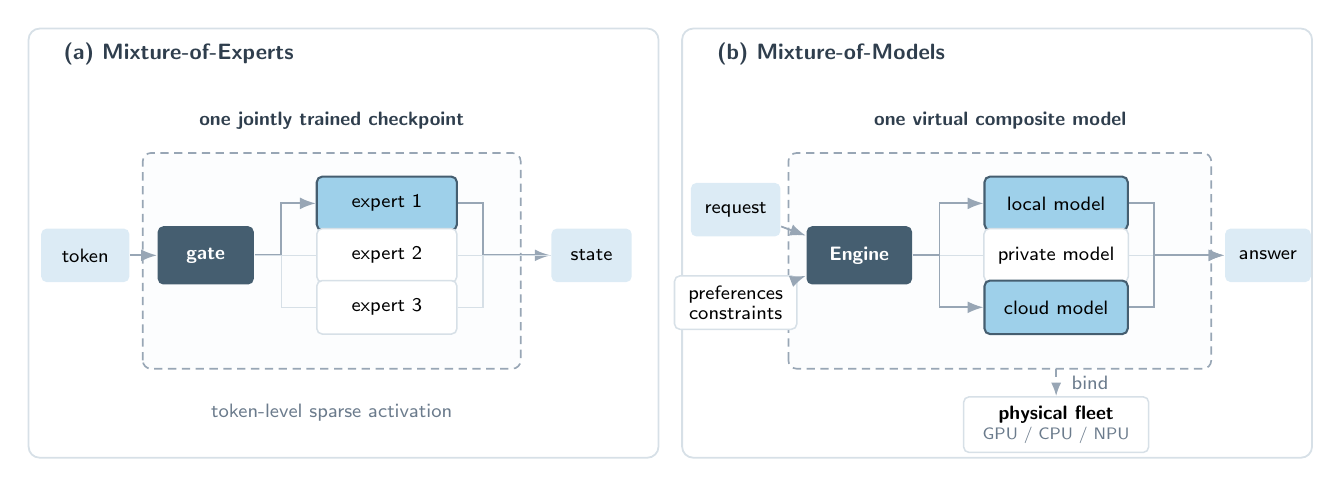
\begin{tikzpicture}[
  x=1cm,y=1cm,font=\sffamily,>=Latex,
  flow/.style={-{Latex[length=2.0mm]},draw=MoMGray,line width=0.65pt},
  bind/.style={-{Latex[length=1.7mm]},draw=MoMGray,densely dashed,line width=0.55pt},
  boundary/.style={draw=MoMGray,fill=MoMBlueLight!9,densely dashed,
    rounded corners=3pt,line width=0.6pt},
  card/.style={draw=MoMBorder,fill=white,rounded corners=2pt,line width=0.55pt,
    minimum height=0.68cm,inner xsep=5pt,align=center,
    font=\sffamily\fontsize{7.2}{8.1}\selectfont},
  soft/.style={card,draw=none,fill=MoMBlueLight},
  core/.style={card,draw=none,fill=MoMDark,text=white,
    minimum height=0.74cm,font=\sffamily\bfseries\fontsize{7.2}{8.1}\selectfont},
  active/.style={card,draw=MoMDark,fill=MoMBlue,line width=0.75pt},
  tiny/.style={font=\sffamily\fontsize{6.7}{7.5}\selectfont,text=MoMMuted},
  grouptitle/.style={font=\sffamily\bfseries\fontsize{7.1}{8.0}\selectfont,
    text=MoMText},
  paneltitle/.style={font=\sffamily\bfseries\fontsize{8.4}{9.4}\selectfont,
    text=MoMText}
]

% Symmetric panels compare the two loci of conditional computation.
\draw[draw=MoMBorder,rounded corners=4pt,line width=0.65pt]
  (0,0.15) rectangle (8.0,5.60);
\draw[draw=MoMBorder,rounded corners=4pt,line width=0.65pt]
  (8.30,0.15) rectangle (16.30,5.60);
\node[paneltitle,anchor=west] at (0.32,5.28) {(a) Mixture-of-Experts};
\node[paneltitle,anchor=west] at (8.62,5.28) {(b) Mixture-of-Models};

% MoE: gate and experts share one training and checkpoint boundary.
\draw[boundary] (1.45,1.28) rectangle (6.25,4.02);
\node[grouptitle] at (3.85,4.43) {one jointly trained checkpoint};

\node[soft,minimum width=1.12cm] (token) at (0.72,2.72) {token};
\node[core,minimum width=1.22cm] (gate) at (2.25,2.72) {gate};
\node[active,minimum width=1.78cm] (e1) at (4.55,3.38) {expert 1};
\node[card,minimum width=1.78cm] (e2) at (4.55,2.72) {expert 2};
\node[card,minimum width=1.78cm] (e3) at (4.55,2.06) {expert 3};
\node[soft,minimum width=1.02cm] (state) at (7.15,2.72) {state};

\draw[flow] (token) -- (gate);
\draw[flow] (gate.east) -- ++(0.34,0) |- (e1.west);
\draw[draw=MoMBorder,line width=0.45pt] (gate.east) -- ++(0.34,0) |- (e2.west);
\draw[draw=MoMBorder,line width=0.45pt] (gate.east) -- ++(0.34,0) |- (e3.west);
\draw[flow] (e1.east) -- ++(0.32,0) |- (state.west);
\draw[draw=MoMBorder,line width=0.45pt] (e2.east) -- ++(0.32,0) |- (state.west);
\draw[draw=MoMBorder,line width=0.45pt] (e3.east) -- ++(0.32,0) |- (state.west);
\node[tiny] at (3.85,0.72) {token-level sparse activation};

% MoM: engine and constituent models form the complete virtual model.
\draw[boundary] (9.65,1.28) rectangle (15.02,4.02);
\node[grouptitle] at (12.34,4.43) {one virtual composite model};

\node[soft,minimum width=1.12cm] (request) at (8.98,3.30) {request};
\node[card,minimum width=1.22cm] (profile) at (8.98,2.12)
  {preferences\\[-1pt]constraints};
\node[core,minimum width=1.34cm] (engine) at (10.55,2.72) {Engine};
\node[active,minimum width=1.82cm] (m1) at (13.05,3.38) {local model};
\node[card,minimum width=1.82cm] (m2) at (13.05,2.72) {private model};
\node[active,minimum width=1.82cm] (m3) at (13.05,2.06) {cloud model};
\node[soft,minimum width=1.08cm] (answer) at (15.74,2.72) {answer};

\draw[flow] (request) -- (engine);
\draw[flow] (profile) -- (engine);
\draw[flow] (engine.east) -- ++(0.34,0) |- (m1.west);
\draw[draw=MoMBorder,line width=0.45pt] (engine.east) -- ++(0.34,0) |- (m2.west);
\draw[flow] (engine.east) -- ++(0.34,0) |- (m3.west);
\draw[flow] (m1.east) -- ++(0.32,0) |- (answer.west);
\draw[draw=MoMBorder,line width=0.45pt] (m2.east) -- ++(0.32,0) |- (answer.west);
\draw[flow] (m3.east) -- ++(0.32,0) |- (answer.west);

% Physical resources remain outside the logical composite-model boundary.
% A single realization card keeps the logical-to-physical edge unambiguous.
\node[card,minimum width=2.35cm,minimum height=0.58cm] (fleet) at (13.05,0.57)
  {{\bfseries physical fleet}\\[-1pt]
   {\fontsize{6.3}{7.0}\selectfont\color{MoMMuted} GPU / CPU / NPU}};
\draw[bind] (13.05,1.28) -- node[tiny,anchor=west,xshift=2pt] {bind} (fleet.north);

\end{tikzpicture}
}
  \caption{\textbf{Conditional computation at two model boundaries.} In MoE,
  a gate selects experts inside one jointly trained checkpoint. In MoM, an
  engine selects and composes independently versioned models behind one model
  interface; a deployment binding maps their logical identities onto a physical
  fleet. Highlighted nodes show one realized trace.}
  \label{fig:moe-vs-mom}
\end{figure}

Crossing the model boundary changes the optimization object. MoM does not
require a shared parameter space. Instead, it learns or searches over
admissible traces, then promotes changes to control state, pools, topology,
contracts, or deployment as explicit revisions. Candidates are evaluated on
realized utility and constraint outcomes. Uniform utilization is not an
intrinsic goal because constituents differ in capability, price, capacity, and
policy eligibility.

This paper makes three contributions:
\begin{itemize}
  \item We formalize MoM as a preference-conditioned distribution over finite,
  typed execution traces, separating hard admissibility from soft objectives
  and defining capacity diagnostics and failure criteria.
  \item We specify a composite-model format and lifecycle from logical
  specification to portable bundle, realization profile, environment binding,
  resolution lock, and attributable execution.
  \item We ground the execution and systems claims with released multi-model
  runs and a routing-aware capacity case study, and state the matched-budget
  tests required to establish conditional scaling.
\end{itemize}

\section{Mixture-of-Models as a Model Architecture}
\label{sec:formalism}

\subsection{One model beyond one checkpoint}

In conventional deployments, a model name resolves to one checkpoint or managed
endpoint. A Mixture-of-Models (MoM) instead exposes one model interface while
computation crosses model, provider, process, and device boundaries. Its
components may be open or closed, local or remote, and independently versioned
and invoked; they are typically, but need not be, independently trained.
Its model identity is defined not by shared weights but by a versioned
executable specification that fixes logical references, admissible
substitutions, composition, constraints, and the output contract.

Each published model fixes a behavior variant $b$, its default objective, and
an allowed domain $\mathcal{U}_b$ of request preferences. For an input $x$,
conversation or session history $h$, request preference $u\in\mathcal{U}_b$,
and observable environment state $e$, we define its logical specification as
\begin{equation}
  \mathcal{M}_b =
  (\mathcal{V}, \mathcal{Q}, \mathcal{U}_b, S_{\phi}, P_{\omega}, \pi_{\psi},
   \mathcal{A}, \mathcal{G}, \mathcal{K}, \Gamma).
  \label{eq:mom-object}
\end{equation}
Here $\mathcal{V}=\{v_1,\ldots,v_n\}$ contains \emph{logical model references},
not URLs; each declares an exact identity or capability requirement together
with interfaces and deployment requirements. Optional $\mathcal{Q}$ contains
declared typed auxiliary operators for retrieval, tool use, and other bounded
effects; operators have the same explicit interface, policy, and provenance
requirements as model calls, while persistent application state remains
outside the model. $\mathcal{U}_b$ contains the typed request preferences and
policy refinements admitted by behavior variant $b$; it cannot override a hard
guard or transform one published variant into another.
$S_{\phi}$ extracts typed signals such as domain, complexity, modality, risk,
and confidence; $P_{\omega}$ projects them to calibrated scores and predicates;
and $\pi_{\psi}$ chooses the next admissible action. $\mathcal{A}$ defines
action and transition semantics, $\mathcal{G}$ contains typed preconditions and
postconditions, $\mathcal{K}$ defines intermediate and final contracts, and
$\Gamma$ imposes finite bounds on events, path length, fan-out, calls, rounds,
tokens, and time. These components may be learned or authored; content-addressed
prompts and policy assets parameterize the specification. Catalogs, topologies,
prompts, thresholds, contracts, and bounds can be optimized even without
gradients through a constituent model.

A deployment binding later resolves a logical requirement to a local checkpoint
or provider model. Thus the specification can be inspected and packaged without
credentials, then rebound without editing its decision semantics
(Section~\ref{sec:artifact}). We write
$\mathcal{R}=(\mathcal{M}_b,\mathcal{B},L)$ for a \emph{deployed MoM}, where
$\mathcal{B}$ is the environment binding and $L$ is the completed resolution
lock, including the engine revision. Logical identity belongs to $\mathcal{M}_b$.
The caller observes $\mathcal{R}$ as one virtual model: the engine revision
recorded in $L$ executes $\mathcal{M}_b$ against the resolved pool, producing an
attributed event DAG for each request. This distinction permits cross-engine
portability without reducing the deployed model to either the engine or its
endpoints.

\subsection{Execution-trace semantics}

Before event $j$, the runtime state is
\begin{equation}
  \xi_j=(x,h,u,e,z_j,m_j,b_j), \qquad
  z_j=P_{\omega}(S_{\phi}(x,h,e,m_j),h,u,e,m_j),
\end{equation}
where $m_j$ is typed working memory and $b_j$ is the remaining resource budget.
Recomputing $z_j$ allows later decisions to use validated outputs from earlier
events without granting a planner unbounded control.
The primitive actions are
\begin{equation}
\begin{split}
  \textsc{Call}(v,r),\quad &\textsc{Op}(q,r),\quad
  \textsc{Fork}(a_1,\ldots,a_k),\\
  \textsc{Join}(f),\quad &\textsc{Check}(k),\quad
  \textsc{Transform}(f),\quad
  \textsc{Return}(s,y).
\end{split}
\label{eq:actions}
\end{equation}
A call invokes $v$ with a checked request; $\textsc{Op}$ invokes a declared,
typed external operator $q$ such as retrieval or a tool; fork and join implement
bounded parallel composition; check evaluates a guard; and transform is typed
and deterministic.  Planners and judges are ordinary calls, not sources of
unbounded control flow. Every terminal trace ends with a typed status
$s\in\{\texttt{ok},\texttt{abstain},\texttt{reject},\texttt{error}\}$; for a
non-answer status, $y=\bot$. Let $\bar y=(s,y)$ denote the complete terminal
outcome.

An execution trace is a finite, labeled event DAG
\begin{equation}
  \tau=(N,\prec,\sigma,\{(\xi_j,a_j,o_j)\}_{j\in N},\bar y),
  \label{eq:trace}
\end{equation}
where $N$ is the event set, $\prec$ is the control-and-data happens-before
relation, and $\sigma$ is a canonical topological order used only for logging
and replay. A sequential trace has a total order; \textsc{Fork} creates
incomparable child regions, and \textsc{Join} depends on their terminal events.
Stable branch identifiers make $\sigma$ unique, so different interleavings do
not create duplicate traces. The state $\xi_j$ is a deterministic function of
the outcomes visible through predecessors of $j$; wall-clock observations and
timeouts remain part of $e$ and $o_j$. Both $|N|$ and every path length are
finite under $\Gamma$.

The policy may be stochastic and condition on prior model outputs through
$m_j$. Let $L$ identify the bound constituent revisions, let $C(\tau)\subseteq
N$ contain the controller's choice events, and let $E(\tau)\subseteq N$ contain
effectful model and operator calls. Graph-prescribed and administrative events
have unit probability. For event $j$, the causal history
$H_j=\{o_k:k\prec j\}$ contains only predecessor-visible outcomes; $\xi_j$ is
measurable with respect to this history. In particular, a branch cannot observe
an incomparable branch before their declared join.

Parallel calls can share provider, load, and runtime randomness, so we do not
assume that their outcomes are conditionally independent. Instead, let
$K_L$ be the causal execution kernel over all effectful outcomes for the chosen
action DAG, and let $r_{E(\tau)}$ collect the checked requests attached to its
effectful actions. The joint probability of a valid trace and terminal outcome is
\begin{equation}
\begin{aligned}
 p_{\mathcal{R}}(\bar y,\tau\mid x,h,u,e)
 ={}& \mathbf{1}[\textsc{Return}(\tau)=\bar y]
      \prod_{j\in C(\tau)}\pi_{\psi}(a_j\mid\xi_j)\\
 &\cdot K_L\!\left(o_{E(\tau)}\mid r_{E(\tau)},a_{E(\tau)},
                   \prec,x,h,u,e\right).
\end{aligned}
\label{eq:trace-factorization}
\end{equation}
The kernel is causal: an event distribution may depend on $H_j$ and shared
runtime state, but not on incomparable or future outcomes. When effectful calls
are conditionally independent given their causal histories, $K_L$ reduces to a
product of per-call response kernels. The user-facing distribution of the
deployed realization marginalizes admissible event DAGs,
\begin{equation}
 p_{\mathcal{R}}(\bar y\mid x,h,u,e)
 = \sum_{\tau\in\mathcal{T}_{\mathrm{adm}}}
   p_{\mathcal{R}}(\bar y,\tau\mid x,h,u,e).
 \label{eq:mom-distribution}
\end{equation}
Closed-model token probabilities need not be accessible: training may use
sampled outputs, scores, preferences, or outcomes.

The trace view unifies common structures.  \textbf{Selection} calls one model;
a \textbf{cascade} conditionally escalates through an ordered sequence;
\textbf{fusion} forks a bounded panel and joins its responses;
\textbf{multi-round collaboration} repeats calls over typed shared state; and a
\textbf{workflow} instantiates a bounded static graph or validated planner
output.  Routing is therefore one MoM topology, while a collection of APIs is
not a MoM until its admissible traces, contracts, and identity are explicit.
Fixed panels and workflows are degenerate policies that assign probability one
to one graph; conditional computation does not require every trace to activate
a strict subset of the catalog.

\begin{figure}[H]
  \centering
  \resizebox{\linewidth}{!}{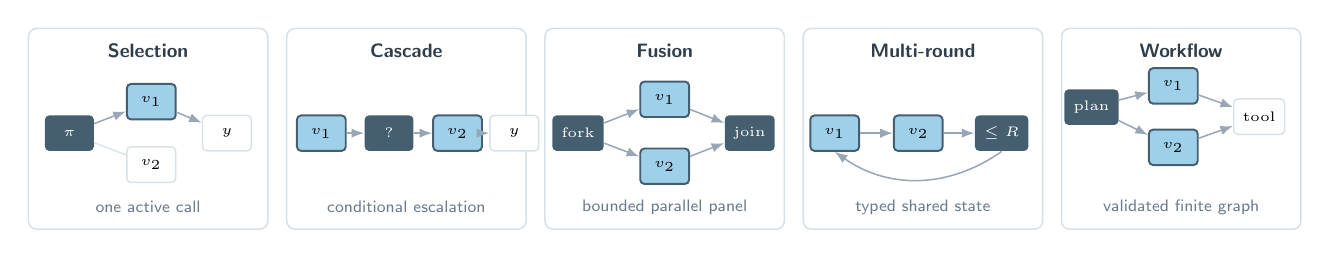
\begin{tikzpicture}[
  x=1cm,y=1cm,font=\sffamily,>=Latex,
  edge/.style={-{Latex[length=1.6mm]},draw=MoMGray,line width=0.55pt},
  call/.style={draw=MoMBorder,fill=white,rounded corners=1.5pt,line width=0.5pt,minimum width=0.62cm,minimum height=0.45cm,font=\tiny},
  selected/.style={draw=MoMDark,fill=MoMBlue,rounded corners=1.5pt,line width=0.7pt,minimum width=0.62cm,minimum height=0.45cm,font=\tiny},
  control/.style={draw=none,fill=MoMDark,text=white,rounded corners=1.5pt,minimum width=0.62cm,minimum height=0.45cm,font=\tiny},
  panel/.style={draw=MoMBorder,rounded corners=3pt,line width=0.55pt},
  title/.style={font=\sffamily\bfseries\fontsize{7.0}{8}\selectfont,text=MoMText},
  note/.style={font=\sffamily\fontsize{5.8}{6.7}\selectfont,text=MoMMuted}
]
\foreach \x/\name in {0/Selection,3.28/Cascade,6.56/Fusion,9.84/Multi-round,13.12/Workflow}{
  \draw[panel] (\x,0) rectangle ++(3.04,2.55);
  \node[title] at (\x+1.52,2.27) {\name};
}

% Selection.
\node[control] (s0) at (0.52,1.22) {$\pi$};
\node[selected] (s1) at (1.56,1.62) {$v_1$};
\node[call] (s2) at (1.56,0.82) {$v_2$};
\node[call] (s3) at (2.52,1.22) {$y$};
\draw[edge] (s0) -- (s1);
\draw[draw=MoMBorder,line width=0.45pt] (s0) -- (s2);
\draw[edge] (s1) -- (s3);
\node[note] at (1.52,0.28) {one active call};

% Cascade.
\node[selected] (c1) at (3.72,1.22) {$v_1$};
\node[control] (ck) at (4.58,1.22) {?};
\node[selected] (c2) at (5.45,1.22) {$v_2$};
\node[call] (cy) at (6.17,1.22) {$y$};
\draw[edge] (c1) -- (ck);
\draw[edge] (ck) -- (c2);
\draw[edge] (c2) -- (cy);
\node[note] at (4.80,0.28) {conditional escalation};

% Fusion.
\node[control] (f0) at (6.98,1.22) {fork};
\node[selected] (f1) at (8.08,1.65) {$v_1$};
\node[selected] (f2) at (8.08,0.80) {$v_2$};
\node[control] (fj) at (9.16,1.22) {join};
\draw[edge] (f0) -- (f1);
\draw[edge] (f0) -- (f2);
\draw[edge] (f1) -- (fj);
\draw[edge] (f2) -- (fj);
\node[note] at (8.08,0.28) {bounded parallel panel};

% Multi-round.
\node[selected] (r1) at (10.24,1.22) {$v_1$};
\node[selected] (r2) at (11.30,1.22) {$v_2$};
\node[control] (rb) at (12.36,1.22) {$\leq R$};
\draw[edge] (r1) -- (r2);
\draw[edge] (r2) -- (rb);
\draw[edge] (rb.south) to[bend left=35] (r1.south);
\node[note] at (11.36,0.28) {typed shared state};

% Workflow.
\node[control] (w0) at (13.50,1.55) {plan};
\node[selected] (w1) at (14.54,1.82) {$v_1$};
\node[selected] (w2) at (14.54,1.04) {$v_2$};
\node[call] (w3) at (15.63,1.43) {tool};
\draw[edge] (w0) -- (w1);
\draw[edge] (w0) -- (w2);
\draw[edge] (w1) -- (w3);
\draw[edge] (w2) -- (w3);
\node[note] at (14.64,0.28) {validated finite graph};
\end{tikzpicture}
}
  \caption{\textbf{One trace semantics, multiple execution topologies.}
  Selection, conditional cascades, bounded parallel fusion, multi-round
  collaboration, and validated workflows use the same primitive actions and
  resource bounds.  Blue nodes are calls realized in the illustrated trace;
  white nodes remain admissible but inactive.}
  \label{fig:trace-topologies}
\end{figure}

\paragraph{Coverage of bounded graphs.}
The action vocabulary is designed to represent finite, well-typed control-flow graphs
whose effectful vertices call members of $\mathcal{V}\cup\mathcal{Q}$, whose
branches and joins have declared semantics, and whose cycles have finite bounds.
Model and operator vertices map to \textsc{Call} and \textsc{Op}; branches to
\textsc{Check} and policy transitions; parallel regions to
\textsc{Fork}/\textsc{Join}; deterministic vertices to \textsc{Transform}; and
terminals to \textsc{Return}. Bounded cycles can be unrolled or represented by
a counter in typed memory. For fixed binding, response kernels, and scheduler
semantics, the translation preserves typed terminal outcomes and effectful
calls up to deterministic administrative steps under these declared
assumptions. This is a design property, not a claim that every graph can be
learned efficiently. It lets
selection, cascades, panels, multi-round protocols, and finite workflows share
one runtime action vocabulary.

\subsection{Preferences define objectives; policies must satisfy constraints}
\label{sec:objectives}

Let $R(\bar y,y^*)$ measure task utility, including the utility of explicit
abstention, rejection, or error, and let
$c(\tau,e)\in\mathbb{R}_{+}^{d}$ contain soft resource outcomes such as monetary
cost, latency, generated tokens, energy use, and estimated emissions. A
request preference $u$ compiles to weights $\lambda(u)$ and, where appropriate,
targets or service-level objectives.  For a data distribution $\mathcal{D}$, a
basic training objective is
\begin{equation}
 \max_{\Theta}
 \;\mathbb{E}_{(x,h,u,e,y^*)\sim\mathcal{D},\,
 \tau\sim p_{\mathcal{R}_{\Theta}}(\cdot\mid x,h,u,e)}
 \left[R(\bar y,y^*)-\lambda(u)^{\top}c(\tau,e)\right],
 \label{eq:soft-objective}
\end{equation}
where $\Theta=(\theta_{\mathrm{log}},\beta)$ denotes the logical and deployment
coordinates introduced in Section~\ref{sec:optimization}.

Privacy, residency, model allowlists, and capability rules that are known
before a call are typed action preconditions
$g_\ell^{\mathrm{pre}}(\xi_j,a)\in\{0,1,\star\}$, where $\star$ denotes
unknown evidence. They define
\begin{equation}
 \mathcal{A}_{\mathrm{adm}}(\xi_j)
 =\{a\in\mathcal{A}(\xi_j):
 g_\ell^{\mathrm{pre}}(\xi_j,a)=1\;\forall \ell\},
 \qquad
 \pi_\psi(a\mid\xi_j)=0\ \text{if }a\notin\mathcal{A}_{\mathrm{adm}}(\xi_j).
 \label{eq:admissible}
\end{equation}
Only a verified value of $1$ admits an action. The guards cover graph
reachability, artifact policy, environment and binding policy, the selected
behavior variant, and request preference. Either may remove actions from the
environment-admissible set but cannot restore an action excluded by residency,
authorization, or deployment policy.
Postconditions capture properties---such as output validity or grounding---that
can be evaluated only after an action returns. A trace may return \texttt{ok}
only if all postconditions on its realized path hold; otherwise it must take a
declared repair, fallback, abstention, or rejection edge. Thus
$\mathcal{T}_{\mathrm{adm}}\subseteq\mathcal{T}_{\Gamma}$ contains traces whose
actions satisfy Equation~\ref{eq:admissible} and whose failed postconditions
follow declared transitions. If no action is admissible, execution fails closed
with $\textsc{Return}(\texttt{reject},\bot)$. Statistical requirements such as
tail latency should instead use population constraints such as
$\Pr[g_k^{\mathrm{post}}=0]\leq\delta_k$; an unobserved outcome cannot be
filtered before execution.
These guarantees are relative to the declared evidence and checker semantics;
they do not establish confidentiality, safety, or factuality unless those
mechanisms are themselves sound.

Published behavior variants such as \emph{cost-first}, \emph{accuracy-first},
\emph{balanced}, \emph{security-first}, and \emph{grounding-first} fix both
objective defaults and non-negotiable guards, preventing quality from
compensating for a privacy or contract violation. Request preferences may tune
declared tradeoffs only within the selected variant's domain.

Two operating points make the distinction precise. With quality floor $q$,
nonnegative resource weights $w_c$, and expected resource cap $\bar b$, the
same MoM may be optimized as
\begin{equation}
\begin{aligned}
 \text{cost-first:}\quad
 &\min_{\Theta}\ \mathbb{E}[w_c^{\top}c(\tau,e)]
 &&\text{s.t.}\quad \mathbb{E}[R(\bar y,y^*)]\ge q,\\
 \text{accuracy-first:}\quad
 &\max_{\Theta}\ \mathbb{E}[R(\bar y,y^*)]
 &&\text{s.t.}\quad \mathbb{E}[c(\tau,e)]\preceq \bar b.
\end{aligned}
\label{eq:dual-profiles}
\end{equation}
The first uses conditional computation to avoid unnecessary work; the second
uses an expected resource envelope to exploit complementary failure modes.
Per-trace hard limits remain enforced by $\Gamma$. These are first-class
behavior variants with separate versioned coordinates, not application-side
graphs.

\paragraph{Executor contract.}
A conforming executor must make the preceding semantics operational. Given a
well-typed specification, finite event, fan-out, path, and action-duration
bounds, every budget exhaustion, timeout, or stuck state must follow a declared
transition, and execution must eventually terminate within $\Gamma$ with a
typed status. The controller's support must remain inside
$\mathcal{A}_{\mathrm{adm}}(\xi_j)$, and every successful return must be guarded
by its declared postconditions. These obligations yield three checkable runtime
invariants: execution terminates within $\Gamma$ with a typed status; no action
with a false declared precondition is issued; and \texttt{ok} is reachable only
after required checks succeed. They are executor guarantees relative to the
declared guards and evidence, not statistical claims about the correctness of
those guards.

\subsection{Architectural invariants}

Equation~\ref{eq:mom-object} imposes five invariants: execution is
conditionally selected and resource-bounded;
composition is typed; recursion, iteration, and fan-out are bounded; logical
semantics are separate from placement; and every response is attributable to a
MoM version, binding, and trace. These invariants make a MoM optimizable like a
model and operable like a distributed system.

\section{Optimizing and Executing a Mixture-of-Models}
\label{sec:optimization}

MoM extends the optimization surface beyond constituent weights to the
distribution of computation around independently versioned models. A lifecycle
engine can optimize that distribution while preserving one MoM identity across
training, evaluation, and serving. Accordingly, MoM optimization is a
full-stack co-design problem. Changing the trace policy changes the demand
presented to the serving fleet; changing placement, batching, or pool capacity
changes the feasible trace distribution. Logical and physical coordinates must
therefore be optimized jointly while remaining separately versioned for
portability and attribution \citep{chen_2026_wrp}. Figure~\ref{fig:system-codesign}
makes this coupling explicit.

\begin{figure}[H]
  \centering
  \resizebox{\linewidth}{!}{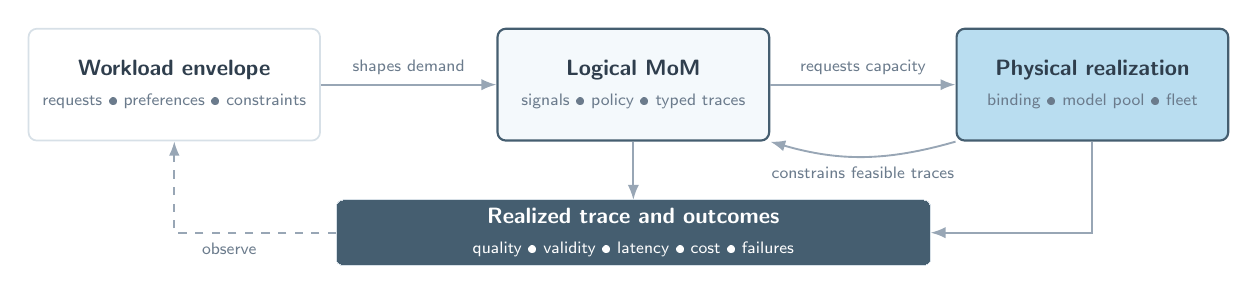
\begin{tikzpicture}[
  x=1cm,y=1cm,font=\sffamily,>=Latex,
  flow/.style={-{Latex[length=1.9mm]},draw=MoMGray,line width=0.68pt},
  feedback/.style={-{Latex[length=1.8mm]},draw=MoMGray,dashed,line width=0.62pt},
  panel/.style={draw=MoMBorder,fill=white,rounded corners=3pt,
    line width=0.62pt,minimum width=3.45cm,minimum height=1.42cm,
    inner xsep=5pt,inner ysep=4pt,align=center,text=MoMText},
  logical/.style={panel,draw=MoMDark,fill=MoMBlueLight!32,line width=0.78pt},
  physical/.style={panel,draw=MoMDark,fill=MoMBlue!72,line width=0.78pt},
  outcome/.style={draw=MoMBorder,fill=MoMDark,text=white,rounded corners=2.6pt,
    line width=0pt,minimum width=7.55cm,minimum height=0.82cm,
    inner xsep=6pt,inner ysep=3pt,align=center},
  meta/.style={font=\sffamily\fontsize{6.5}{7.2}\selectfont,text=MoMMuted}
]

\newcommand{\codesigntitle}{\bfseries\fontsize{8.2}{9.0}\selectfont}
\newcommand{\codesignmeta}{\fontsize{6.5}{7.2}\selectfont\color{MoMMuted}}
\newcommand{\codesignlightmeta}{\fontsize{6.5}{7.2}\selectfont\color{white}}

\node[panel] (workload) at (2.15,2.56)
  {{\codesigntitle Workload envelope}\\[-1pt]
   {\codesignmeta requests \textbullet\ preferences \textbullet\ constraints}};

\node[logical] (logical) at (7.98,2.56)
  {{\codesigntitle Logical MoM}\\[-1pt]
   {\codesignmeta signals \textbullet\ policy \textbullet\ typed traces}};

\node[physical] (physical) at (13.81,2.56)
  {{\codesigntitle Physical realization}\\[-1pt]
   {\codesignmeta binding \textbullet\ model pool \textbullet\ fleet}};

\draw[flow] (workload) -- node[meta,above] {shapes demand} (logical);
\draw[flow] (logical) -- node[meta,above] {requests capacity} (physical);
\draw[flow] (physical.south west) to[bend left=16]
  node[meta,below] {constrains feasible traces} (logical.south east);

\node[outcome] (outcome) at (7.98,0.68)
  {{\codesigntitle Realized trace and outcomes}\\[-1pt]
   {\codesignlightmeta quality \textbullet\ validity \textbullet\ latency
   \textbullet\ cost \textbullet\ failures}};

\draw[flow] (logical.south) -- (outcome.north);
\draw[flow] (physical.south) |- (outcome.east);
\draw[feedback] (outcome.west) -| node[meta,pos=0.33,below] {observe} (workload.south);

\end{tikzpicture}
}
  \caption{\textbf{MoM as system-level intelligence.} Workload, preferences,
  and constraints shape the useful trace distribution; the logical MoM shapes
  demand on constituent models; and bindings, placement, and fleet state bound
  feasible execution. Realized quality, validity, latency, cost, capacity, and
  failures feed back into both logical optimization and physical planning.}
  \label{fig:system-codesign}
\end{figure}

\subsection{Training the trace distribution}

Let $\mathcal{M}_{\theta_{\mathrm{log}}}$ denote a parameterized logical
specification. We write the lifecycle optimization coordinates as
\begin{equation}
 \Theta=(\theta_{\mathrm{log}},\beta),\qquad
 \theta_{\mathrm{log}}=(\phi,\omega,\psi,\rho,\eta),\qquad
 \mathcal{B}=\mathcal{B}_{\beta},\quad
 L=\operatorname{Resolve}(\mathcal{M}_{\theta_{\mathrm{log}}},
                           \mathcal{B}_{\beta},e).
 \label{eq:trainable-surface}
\end{equation}
$\phi$ parameterizes learned signals, $\omega$ their projections, and $\psi$
the action controller. The discrete coordinate $\rho$ selects catalog members,
topology, prompts, thresholds, contracts, and resource bounds already represented
in $\mathcal{M}$; it does not introduce a second semantic authority. Optional
$\eta$ denotes adapters or constituent weights that the optimizer may update.
The deployment coordinate $\beta$ controls binding, placement, replication, and
batching. Promoting $\theta_{\mathrm{log}}$ creates a new logical model version;
changing $\beta$ creates a new binding, after which resolution produces a new
lock.

Different coordinates call for different optimizers. Signals and routes can be
learned from supervision; rankings and escalation from preferences; thresholds
from logged outcomes or bandit feedback; pools and topologies through discrete
search; and prompts and budgets through black-box optimization. The resulting
policy may be distilled into a small controller. Any adapter or
constituent-model fine-tuning must be reported separately.

This definition does not turn every configuration edit into training. A MoM
training procedure must identify its experience source, optimization variables,
held-out objective, constraints, and produced artifact or binding version.
Constituent weights may remain frozen, be tuned independently, or be co-trained
when access and interfaces permit. Online adaptation must additionally bound
exploration and preserve policy invariants.

For a training set, the engine minimizes task loss and soft resource outcomes
subject to the hard admissibility conditions in Equation~\ref{eq:admissible}:
\begin{equation}
\begin{aligned}
 \min_{\Theta}\quad &\frac{1}{N}\sum_{i=1}^{N}
 \mathbb{E}_{\tau\sim p_{\mathcal{R}_{\Theta}}
 (\cdot\mid x_i,h_i,u_i,e_i)}
 \left[\ell(\bar y_i,y_i^*)+\lambda(u_i)^{\top}c(\tau,e_i)\right]\\
 \text{s.t.}\quad &
 \operatorname{supp}p_{\mathcal{R}_{\Theta}}
 (\cdot\mid x_i,h_i,u_i,e_i)\subseteq\mathcal{T}_{\mathrm{adm}}
 \quad\forall i.
\end{aligned}
 \label{eq:mom-training}
\end{equation}
Any allowed statistical violation rate must be stated explicitly and estimated
on held-out data; a soft penalty does not enforce an exact privacy or residency
rule.

Training produces a candidate version or asset, which evaluation compares with
the incumbent under a fixed protocol. Promotion is explicit, and serving never
silently rewrites the active specification. Bounded online adaptation remains
trace-visible and reversible.

\subsection{Capacity is heterogeneous and budgeted}
\label{sec:capacity}

Parameter count is a poor capacity measure: it may be unknown, inactive models
consume no generation compute, and similarly sized models can share errors.
We distinguish \emph{catalog capacity} (capability coverage), \emph{decision
capacity} (complementarity exploitable under a budget), and \emph{serving
capacity} (throughput, memory, concurrency, and failure envelope).

For pure selection and a per-example utility $q_i(x)$ for model $v_i$---with
$h$, $u$, and $e$ suppressed for notation---two diagnostic ceilings are
\begin{equation}
 Q_{\mathrm{single}}=\max_i\mathbb{E}_{x}[q_i(x)],\qquad
 Q_{\mathrm{oracle}}=\mathbb{E}_{x}\left[\max_i q_i(x)\right].
 \label{eq:oracle}
\end{equation}
Their gap $\Delta_{\mathrm{comp}}=Q_{\mathrm{oracle}}-Q_{\mathrm{single}}$
measures selection headroom. Let $Q_{\mathcal{M}}$ be the expected utility of a
pure-selection MoM on the same population and under the same budget. For a
positive gap, controller realization is
\begin{equation}
 \eta_{\mathrm{ctrl}}=
 \frac{Q_{\mathcal{M}}-Q_{\mathrm{single}}}
      {Q_{\mathrm{oracle}}-Q_{\mathrm{single}}}.
 \label{eq:controller-realization}
\end{equation}
Fusion may exceed this oracle because it combines multiple responses; report
that excess separately as composition gain. A large catalog provides little
decision capacity when constituent errors are strongly correlated.

Capacity scaling requires a predeclared matched active-work envelope over
calls, tokens, cost, or latency, with all resource outcomes reported.
Increasing catalog size under that envelope tests conditional capacity;
increasing catalog and active work only tests a larger system.

Let $\mathcal{F}(\mathcal{V},\bar b)$ be the feasible MoM policies over catalog
$\mathcal{V}$ under fixed budget $\bar b$ and fixed constraints, and let
\begin{equation}
 U^*(\mathcal{V},\bar b)=
 \sup_{\pi'\in\mathcal{F}(\mathcal{V},\bar b)}
 \mathbb{E}[R-\lambda^{\top}c].
 \label{eq:catalog-monotonicity}
\end{equation}
If $\mathcal{V}\subseteq\mathcal{V}'$ and every policy feasible over
$\mathcal{V}$ remains feasible over $\mathcal{V}'$, then
$U^*(\mathcal{V}',\bar b)\geq U^*(\mathcal{V},\bar b)$ because a policy over the larger
catalog can assign zero probability to every added model. This monotonicity
belongs to oracle capacity, not to a learned controller. Realized utility may
fall as a catalog grows when controller regret, exploration, or coordination
overhead increases faster than the new complementarity. Separating the benefit
of added complementarity from the cost of controller regret is the central
scaling question.

Let the expected activation of logical model $i$ per request be
\begin{equation}
 \Lambda_i=\mathbb{E}_{\tau}\left[
   \sum_{j\in N}\mathbf{1}[a_j=\textsc{Call}(v_i,\cdot)]\right].
 \label{eq:model-load}
\end{equation}
At request rate $\nu$, $\nu\Lambda_i$ determines its mean call rate. Models differ
in quality, price, limits, and capacity, so uniform $\Lambda_i$ is not a desirable
default.  Balancing should target the highest feasible utility under capacity
and tail-latency constraints, not equal traffic.

\subsection{Collapse and failure modes}

MoM couples statistical and systems failures. \textbf{Pool collapse} is harmful
when concentrated traffic excludes a better feasible policy; route entropy
alone cannot distinguish such collapse from correctly rejecting dominated
models. Diagnose it against $Q_{\mathrm{single}}$, oracle headroom, and realized
utility. \textbf{False complementarity} arises from leakage,
judge bias, or small samples and requires held-out, per-item error correlation.
\textbf{Policy dead zones} leave reachable signal states without valid traces;
static coverage and fail-closed tests expose them.

\textbf{Hidden escalation} underreports cost by omitting retries and fallbacks.
\textbf{Handoff loss} discards context through truncation, poor prompt
translation, or lossy summaries. \textbf{Contract collapse} masks invalid
outputs through unreported repair. Evaluations should therefore trace every
attempt and report first-pass validity, repairs, and terminal failures.

Finally, \textbf{provider drift and capability aliasing} break assumed
substitutability; locks, probes, and continuous evaluation detect and constrain
their effects. \textbf{Placement skew} overloads a pool or violates locality.
Model-generated plans introduce \textbf{unbounded control} unless the engine restricts them to declared
references and enforces $\Gamma$.

\subsection{Compile once, schedule under current state}

Before serving, the proposed engine type-checks the graph, validates contracts
and bounds, and resolves requirements. Per request it evaluates signals, filters
inadmissible actions, applies the preference-conditioned policy, and schedules
the topology.  Parallel latency follows the critical path.  Timeouts, partial
joins, fallbacks, caching, batching, and retries are declared semantics.

The engine emits, alongside each response, a trace linked to the MoM artifact
and resolution lock for attribution, replay, accounting, optimization, and
incident analysis. When policy permits, privacy-preserving redaction should
retain the minimum structural metadata needed to reconstruct the decision.

\paragraph{Reference-engine scope.}
vLLM Semantic Router grounds this execution contract without assuming access
to constituent weights or a jointly differentiable trainer.
Section~\ref{sec:reference-engine} audits the implemented subset and the
lifecycle boundary proposed here.

\section{The Mixture-of-Models Artifact and Lifecycle}
\label{sec:artifact}

A model architecture needs a model artifact, not merely runtime configuration.
For MoM, that artifact is the \emph{bundle}: a typed envelope that gives a
composite model one interface, identity, policy, and finite execution semantics
while leaving constituent checkpoints in their native formats. The same logical
object must remain identifiable across authoring, optimization, evaluation, and
deployment. The bundle carries the logical half of the co-design; binding and
locking instantiate its physical half, and realized traces provide common
evidence for optimizing both. We therefore define six lifecycle stages, separating policy and
learned assets from environment-specific endpoints and traces:
\begin{equation}
 \text{source}\rightarrow\text{typed IR}\rightarrow\text{bundle}
 \rightarrow\text{binding}\rightarrow\text{lock}
 \rightarrow\text{realized trace}.
 \label{eq:artifact-pipeline}
\end{equation}

\begin{figure}[H]
  \centering
  \resizebox{\linewidth}{!}{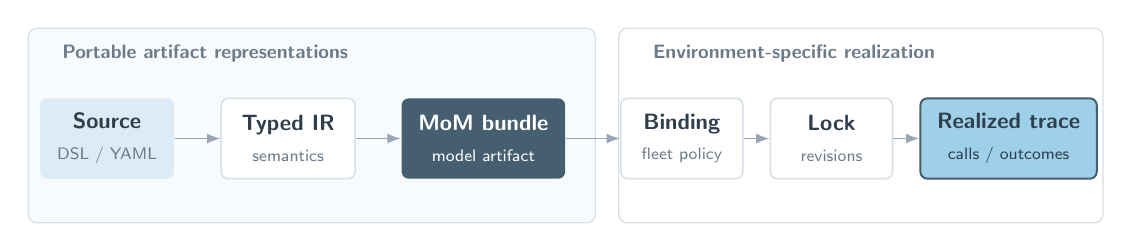
\begin{tikzpicture}[
  x=1cm,y=1cm,font=\sffamily,>=Latex,
  flow/.style={-{Latex[length=1.7mm]},draw=MoMGray,line width=0.65pt},
  group/.style={draw=MoMBorder,fill=white,rounded corners=3pt,line width=0.45pt},
  portable/.style={group,fill=MoMBlueLight!20},
  base/.style={draw=MoMBorder,fill=white,rounded corners=2.5pt,
    line width=0.58pt,minimum height=1.02cm,inner xsep=6pt,
    inner ysep=3pt,align=center,text=MoMText},
  source/.style={base,draw=none,fill=MoMBlueLight},
  bundle/.style={base,draw=none,fill=MoMDark,text=white},
  trace/.style={base,draw=MoMDark,fill=MoMBlue,line width=0.72pt},
  header/.style={font=\sffamily\bfseries\fontsize{7.0}{8.0}\selectfont,
    text=MoMMuted}
]

% Six lifecycle stages share one baseline; the semantic boundary lies between
% the portable bundle and the environment-owned binding.
\draw[portable] (0.05,0.15) rectangle (7.25,2.62);
\draw[group] (7.55,0.15) rectangle (13.70,2.62);
\node[header,anchor=west] at (0.36,2.30) {Portable artifact representations};
\node[header,anchor=west] at (7.86,2.30) {Environment-specific realization};

\node[source,minimum width=1.70cm] (src) at (1.05,1.22)
  {{\bfseries\fontsize{8.0}{8.8}\selectfont Source}\\[-1pt]
   {\fontsize{6.5}{7.2}\selectfont\color{MoMMuted} DSL / YAML}};

\node[base,minimum width=1.70cm] (ir) at (3.35,1.22)
  {{\bfseries\fontsize{8.0}{8.8}\selectfont Typed IR}\\[-1pt]
   {\fontsize{6.5}{7.2}\selectfont\color{MoMMuted} semantics}};

\node[bundle,minimum width=1.95cm] (bundle) at (5.83,1.22)
  {{\bfseries\fontsize{8.0}{8.8}\selectfont MoM bundle}\\[-1pt]
   {\fontsize{6.5}{7.2}\selectfont model artifact}};

\node[base,minimum width=1.55cm] (binding) at (8.35,1.22)
  {{\bfseries\fontsize{8.0}{8.8}\selectfont Binding}\\[-1pt]
   {\fontsize{6.2}{6.9}\selectfont\color{MoMMuted} fleet policy}};

\node[base,minimum width=1.55cm] (lock) at (10.25,1.22)
  {{\bfseries\fontsize{8.0}{8.8}\selectfont Lock}\\[-1pt]
   {\fontsize{6.2}{6.9}\selectfont\color{MoMMuted} revisions}};

\node[trace,minimum width=1.90cm] (realized) at (12.50,1.22)
  {{\bfseries\fontsize{8.0}{8.8}\selectfont Realized trace}\\[-1pt]
   {\fontsize{6.3}{7.0}\selectfont\color{MoMText} calls / outcomes}};

\draw[flow] (src) -- (ir);
\draw[flow] (ir) -- (bundle);
\draw[flow] (bundle) -- (binding);
\draw[flow] (binding) -- (lock);
\draw[flow] (lock) -- (realized);

\end{tikzpicture}
}
  \caption{\textbf{The MoM lifecycle separates portable representation
  from environment-specific realization.} The lifecycle engine compiles source into
  typed IR and an immutable bundle, then binds and resolves logical references
  into a lock. Every realized trace is attributed to the
  bundle, binding, and lock; credentials and live health remain outside the
  portable artifact.}
  \label{fig:artifact-lifecycle}
\end{figure}

\subsection{Six stages, six responsibilities}

The following definitions are normative requirements of the proposed format,
not a description of the current \vsr{} artifact format.

\paragraph{Authoring source.}
Source is a human-readable DSL or YAML with comments, fragments, and
defaults.  Sources that normalize to the same IR define the same logical model.

\paragraph{Canonical typed IR.}
The IR is the semantic authority. It declares schemas and entry points, logical
model requirements, signals and projections, action graphs, extension
interfaces, contracts, behavior variants, request-preference domains, and
bounds. It contains neither credentials
nor implicit defaults. Canonical maps, numbers, and asset references enable
stable hashes and semantic diffs, and unknown fields are rejected. Model
requirements have no competing manifest authority; hard constraints are typed
fail-closed predicates; and every contract check names explicit success and
failure successors.

\paragraph{Portable bundle.}
The bundle is an immutable distribution unit around the IR:
\begin{verbatim}
manifest.json             interface, content index, compatibility
mom.ir.json               canonical executable specification
source/ assets/           authoring sources and semantic assets
contracts/ eval/          schemas and evaluation protocols
targets/ MODEL_CARD.md    realization templates and documentation
\end{verbatim}
Source is optional, allowing an author to export the executable object without
revealing its authoring representation. Leaf artifacts may be safetensors,
ONNX, GGUF, or immutable repository objects; closed constituents remain typed
provider references. Large weights may be external but content-addressed.
Plugin code is not implicitly trusted: the bundle declares an operator set,
interface, effects, and digest; deployment policy allows or rejects it.

A \emph{behavior variant} such as accuracy-first or security-first belongs to
logical semantics and therefore to model identity; it declares the default and
allowed domain of request preferences. A \emph{realization profile}
such as CUDA, ROCm, CPU, edge, or hybrid instead declares portable runtime and
accelerator requirements. It may be distributed with the bundle, but it contains
no endpoint, secret, device identifier, or live capacity and does not change
logical identity.

Backend compatibility is not a scalar \texttt{backend} choice. A binding keeps
six axes distinct: wire transport, API adapter, model runtime, leaf-artifact
format, accelerator, and deployment driver. Thus one admissible trace may use a
ROCm-hosted vLLM model, a CUDA specialist, a CPU verifier, and a managed cloud
API without assigning the composite model itself a single hardware backend.

\paragraph{Deployment binding.}
A binding is an environment-owned mapping
\begin{equation}
 \mathcal{B}:\mathcal{V}\cup\mathcal{Q}\rightarrow 2^{\mathcal{E}}
 \end{equation}
from logical model or operator references to candidate endpoints or local
deployments under a selected realization profile. For
$r\in\mathcal{V}\cup\mathcal{Q}$, each
$d\in \mathcal{B}(r)$ must
satisfy modality, context, capability, data-policy, and interface requirements;
operator candidates also satisfy their declared effect and sandbox
requirements. Bindings declare placement, replicas, limits, prices, and
fallbacks, but contain only secret references. Each candidate exposes its
capability evidence, capacity envelope, and pricing assumptions, so resolution
cannot infer them silently from an endpoint name. Here $\mathcal{E}$ is the
environment's set of candidate deployments.

\paragraph{Resolution lock.}
Resolution lock $L$ records the complete resolved candidate inventory: model,
tokenizer, adapter, image, runtime, accelerator, protocol-adapter, asset, and
plugin identities plus capability evidence. Binding says what may run; lock says
what was resolved; the trace says what actually ran. Revision evidence is typed
as \emph{pinned} when an immutable content or repository identifier can be
recorded and \emph{observed-opaque} when a provider exposes only an alias. The
latter retains an observation time and a content-addressed probe record without
claiming bitwise reproducibility. Floating references are a development mode,
not a production lock.

\paragraph{Realized trace.}
The trace records semantic/bundle/binding/lock digests, behavior variant,
request preference, realization profile, constraint
checks, signals, actions, resolved calls, timing, tokens, usage, accounting
version, realized cost, retries, contracts, and terminal status. Content may be
encrypted, redacted, hashed, or referenced under data policy. A trace is an
observation, not model definition.

\subsection{Identity and portability}

A human coordinate such as \texttt{modelId:version} is not an integrity
identity. We instead separate four content identities. The
\emph{semantic digest} commits to canonical IR and its path-sorted semantic
assets. The \emph{bundle digest} additionally commits to the manifest, source,
contracts, evaluation protocols, target templates, and documentation. The
\emph{binding digest} identifies canonical environment policy, while the
\emph{lock digest} identifies one completed resolution. The manifest stores the
semantic digest; the external lock stores
bundle and binding digests; the lock digest is computed only after the lock is
complete. No object therefore contains its own hash.

Bindings, credentials, and traces are excluded from logical identity.
Rebinding realizes the same logical model but produces new binding and lock
identities; changing a controller, prompt, contract, requirement, behavior
variant, or topology changes the semantic digest. Changing only source
formatting, a model card, or a realization template preserves logical identity
but changes the distributed bundle. Every result carries all four digests.
Together they distinguish semantic,
distribution, environment, and realized-resolution equivalence.

Portability preserves logical and control semantics, not predictive equivalence
across substitutions. It is tested by fixing semantic and bundle digests,
resolving them in two environments, and reporting quality, validity, cost, and
latency under both binding and lock identities. Capability substitutions are
explicit and disclosed; two edited recipes are not portable merely because
they share an API path.

\subsection{Build, import, validation, and export}

Build expands source defaults into canonical IR and performs four classes of
checks: schema and type validity; reference, reachability, and bound
correctness; well-formed contract branches and statically decidable constraint
consistency; and path, digest, and license-record integrity. Explicit migration
handles older source versions; runtime evidence resolves guards that cannot be
decided statically. Import instead verifies an already built artifact, records
its content identity, and never recompiles an optional source representation.
At deployment, every reachable call needs an admissible binding or a declared
fallback or abstention path.

Export writes canonical IR, a deterministic manifest, content-addressed assets,
and evaluation protocols---never credentials, endpoint health, online counters,
or private traces. It may produce a thin artifact of pinned references, a
materialized artifact containing redistributable leaf objects, or a targeted
artifact with selected runtime objects. Materialization fails rather than
pretending that a closed provider is portable. Source round-tripping preserves
semantics, not formatting. IR diff reports behavior changes such as a widened
candidate set or relaxed residency guard.

Consumers verify digests, schemas, operator sets, and engine capabilities;
deployment policy
enforces plugin and license rules and probes model access. Evaluation results,
build provenance, SBOMs, and signatures are digest-bound attestations outside
the bundle, so new evidence does not redefine the evaluated model.

This boundary follows useful precedents without reducing MoM to any one of
them. Hugging Face repositories motivate a save/load model coordinate and
immutable revision pinning; MLflow motivates signatures shared by loading,
serving, and evaluation; ONNX separates a versioned logical IR from
capability-negotiated execution providers; and OCI supplies content-addressed
descriptors and distribution primitives
\citep{huggingface_2026_models,mlflow_2026_model_format,
onnx_2026_ir,onnxruntime_2026_execution_providers,oci_2025_image_spec}.
MoM applies this separation at the model-call level: an accelerator or runtime
realizes the model but does not define it.

\subsection{One lifecycle across training, evaluation, and inference}

An optimizer consumes data or traces from a deployed realization
$(\mathcal{M}_k,\mathcal{B}_k,L_k)$ and emits a complete logical or binding
candidate, not an opaque mutation. Under recorded resolution locks, evaluation
compares candidate and incumbent on quality, violations, cost, latency, retries,
and uncertainty before promotion. Serving emits traces, monitoring detects
drift, replay reconstructs decisions, and approved traces feed offline
optimization. Immutable local revisions support revision-pinned re-execution;
stochastic sampling and runtime scheduling still require recorded seeds and
events. Opaque provider aliases support attributed re-evaluation and drift
measurement, not bitwise reproduction.

Online adaptation may update trace-linked local state, but the model changes
only when that state is promoted into a hashed asset or IR revision.  Session
protection and fallback remain runtime state, preventing one replica's traffic
from silently redefining another's artifact.

\section{An Execution Substrate for Mixture-of-Models}
\label{sec:reference-engine}

\vsr{}\footnote{Open-source implementation:
\url{https://github.com/vllm-project/semantic-router}.} provides an initial
execution substrate for MoM. Current releases expose selection and bounded
multi-model policies through standard model APIs, driven by typed request
analysis and declared model references, with evaluation and replay hooks around
the resulting decision. This demonstrates that heterogeneous model identities
and multi-call topologies can execute behind one model invocation rather than
inside an agent harness. The portable bundle, environment-owned binding and
lock, topology-neutral interpreter, and canonical event DAG proposed in
Section~\ref{sec:artifact} remain lifecycle extensions rather than shipped
features.

\begin{figure}[htbp]
  \centering
  \resizebox{0.98\linewidth}{!}{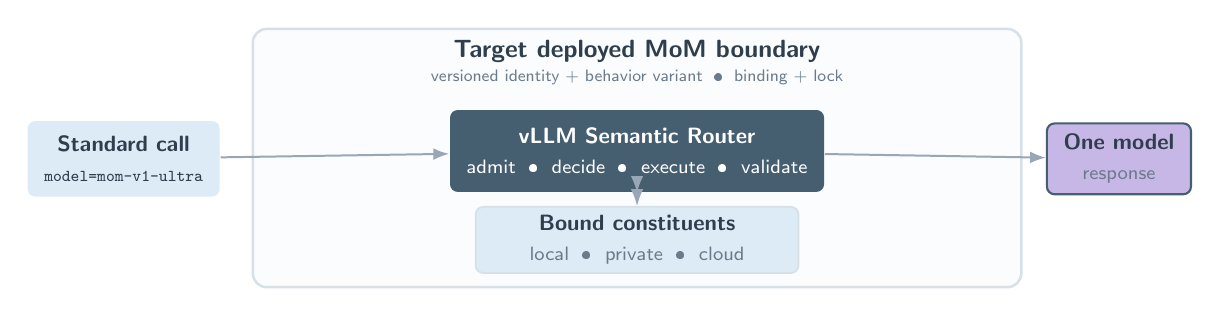
\begin{tikzpicture}[
  x=1cm,y=1cm,font=\sffamily,>=Latex,
  flow/.style={-{Latex[length=2.0mm]},draw=MoMGray,line width=0.72pt},
  exchange/.style={<->,>=Latex,draw=MoMGray,line width=0.68pt},
  boundary/.style={draw=MoMBorder,fill=MoMBlueLight!13,rounded corners=5pt,
    line width=0.9pt},
  box/.style={draw=MoMBorder,fill=white,rounded corners=2.8pt,
    line width=0.64pt,minimum height=0.86cm,inner xsep=6pt,
    inner ysep=3pt,align=center,text=MoMText},
  dark/.style={box,draw=none,fill=MoMDark,text=white},
  identity/.style={box,draw=none,fill=MoMBlueLight},
  response/.style={box,draw=MoMDark,fill=MoMPurple,line width=0.76pt},
  title/.style={font=\sffamily\bfseries\fontsize{9.5}{10.3}\selectfont,
    text=MoMText},
  meta/.style={font=\sffamily\fontsize{6.5}{7.2}\selectfont,text=MoMMuted}
]

\newcommand{\momfigmain}{\bfseries\fontsize{8.2}{9.0}\selectfont}
\newcommand{\momfigsub}{\fontsize{6.7}{7.4}\selectfont\color{MoMMuted}}
\newcommand{\momfiglightsub}{\fontsize{6.7}{7.4}\selectfont\color{white}}

% One proposition: a standard model call crosses a single deployed MoM
% boundary containing both the lifecycle engine and its bound constituents.
\draw[boundary] (3.02,0.82) rectangle (12.78,4.10);
\node[title] at (7.90,3.82) {Target deployed MoM boundary};
\node[meta] at (7.90,3.48)
  {versioned identity + behavior variant \;\textbullet\; binding + lock};

\node[identity,minimum width=2.35cm,minimum height=0.96cm] (request) at (1.38,2.45)
  {{\bfseries\fontsize{8.0}{8.8}\selectfont Standard call}\\[-1pt]
   {\fontsize{6.3}{7.0}\selectfont\ttfamily model=mom-v1-ultra}};

\node[dark,minimum width=4.35cm,minimum height=1.04cm] (engine) at (7.90,2.55)
  {{\momfigmain vLLM Semantic Router}\\[-1pt]
   {\momfiglightsub admit \;\textbullet\; decide \;\textbullet\; execute \;\textbullet\; validate}};

\node[response,minimum width=1.75cm,minimum height=0.90cm] (answer) at (14.02,2.45)
  {{\momfigmain One model}\\[-1pt]{\momfigsub response}};

\draw[flow] (request) -- (engine);
\draw[flow] (engine) -- (answer);

\node[box,fill=MoMBlueLight,draw=MoMBorder,minimum width=4.10cm,
  minimum height=0.80cm] (pool) at (7.90,1.42)
  {{\momfigmain Bound constituents}\\[-1pt]
   {\momfigsub local \;\textbullet\; private \;\textbullet\; cloud}};

\draw[exchange] (engine.south) -- (pool.north);

\end{tikzpicture}
}
  \caption{\textbf{The model-invocation boundary of a deployed MoM.} A caller
  issues one standard model request and receives one response, while the engine
  admits, composes, and observes bounded calls to bound constituents. Current
  provider mappings resolve configured names to backend targets. Portable
  identity and environment-specific resolution complete the proposed lifecycle
  boundary.}
  \label{fig:reference-engine}
\end{figure}

\subsection{Why the control point is below agents}

An agent runtime owns application semantics: goals, task decomposition,
interaction state, and the intent to invoke a model. A MoM engine owns a
different contract: whether model-level computation is admissible, how it is
resolved and scheduled, which finite budget it may consume, and how the result
is attributed. The model-invocation boundary is the narrowest common seam at
which this contract can cover direct inference, retrieval-augmented generation,
agent loops, batch jobs, and embedded systems without depending on one agent
framework.

At this seam, a complete engine can enforce authorization and residency,
resolve logical references against deployment evidence, reserve budgets, choose
legal fallbacks, and account for every attempt. Current \vsr{} implements only
part of that contract; the full admissibility and attribution boundary belongs
to the proposed MoM format. When deployed as the exclusive model ingress,
this placement prevents direct calls from bypassing policy and avoids
reproducing governance logic in every agent harness.

The boundary remains closed-world: one invocation must use only declared models
and operators, consume finite resources, and return one terminal response.
An agent may invoke a MoM or request a bounded workflow, but persistent goals,
task queues, and application state remain outside the logical model. Agents are
clients of the model infrastructure, not its portability or accounting
boundary.

Figure~\ref{fig:deployment-envelopes} shows why this placement matters. One
logical MoM can retain its interface, graph, preferences, and constraints while
different bindings realize it on a robot, at an edge site, in a sovereign data
center, or through managed cloud services.

\begin{figure}[htbp]
  \centering
  \resizebox{\linewidth}{!}{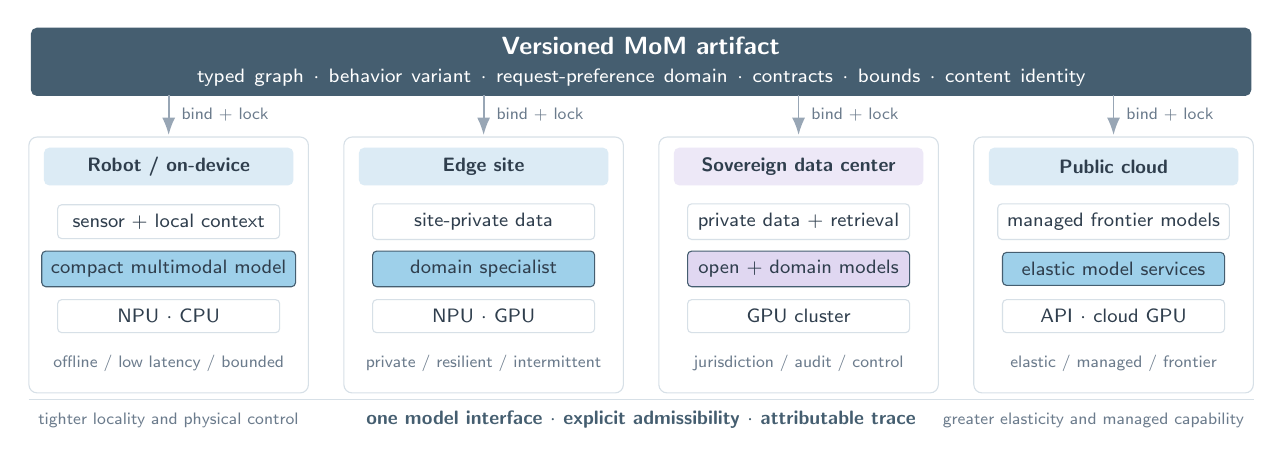
\begin{tikzpicture}[
  x=1cm,
  y=1cm,
  >=Latex,
  artifact/.style={
    draw=MoMDark,
    fill=MoMDark,
    text=white,
    rounded corners=2pt,
    minimum height=0.82cm,
    text width=15.25cm,
    align=center,
    font=\sffamily\bfseries\small
  },
  panel/.style={
    draw=MoMBorder,
    fill=white,
    rounded corners=3pt,
    minimum width=3.55cm,
    minimum height=3.25cm
  },
  paneltitle/.style={
    draw=none,
    fill=MoMBlueLight,
    rounded corners=2pt,
    minimum width=3.17cm,
    minimum height=0.48cm,
    align=center,
    font=\sffamily\bfseries\scriptsize,
    text=MoMText
  },
  component/.style={
    draw=MoMBorder,
    fill=white,
    rounded corners=1.5pt,
    minimum width=2.82cm,
    minimum height=0.42cm,
    align=center,
    font=\sffamily\scriptsize,
    text=MoMText
  },
  active/.style={
    component,
    draw=MoMDark,
    fill=MoMBlue
  },
  note/.style={
    align=center,
    font=\sffamily\fontsize{6.1}{6.8}\selectfont,
    text=MoMMuted
  },
  bind/.style={
    -{Latex[length=2.2mm]},
    draw=MoMGray,
    line width=0.65pt
  }
]

\node[artifact] (artifact) at (8.0,5.05)
  {Versioned MoM artifact\\[-1pt]
   \mdseries\scriptsize typed graph $\cdot$ behavior variant $\cdot$ request-preference domain
   $\cdot$ contracts $\cdot$ bounds $\cdot$ content identity};

\foreach \x in {2.0,6.0,10.0,14.0} {
  \draw[bind] (\x,4.63) -- node[right=1pt,note] {bind + lock} (\x,4.12);
}

\node[panel] at (2.0,2.47) {};
\node[paneltitle] at (2.0,3.72) {Robot / on-device};
\node[component] at (2.0,3.02) {sensor + local context};
\node[active] at (2.0,2.42) {compact multimodal model};
\node[component] at (2.0,1.82) {NPU $\cdot$ CPU};
\node[note] at (2.0,1.22) {offline / low latency / bounded};

\node[panel] at (6.0,2.47) {};
\node[paneltitle] at (6.0,3.72) {Edge site};
\node[component] at (6.0,3.02) {site-private data};
\node[active] at (6.0,2.42) {domain specialist};
\node[component] at (6.0,1.82) {NPU $\cdot$ GPU};
\node[note] at (6.0,1.22) {private / resilient / intermittent};

\node[panel] at (10.0,2.47) {};
\node[paneltitle,fill=MoMPurple!32] at (10.0,3.72) {Sovereign data center};
\node[component] at (10.0,3.02) {private data + retrieval};
\node[active,fill=MoMPurple!55] at (10.0,2.42) {open + domain models};
\node[component] at (10.0,1.82) {GPU cluster};
\node[note] at (10.0,1.22) {jurisdiction / audit / control};

\node[panel] at (14.0,2.47) {};
\node[paneltitle] at (14.0,3.72) {Public cloud};
\node[component] at (14.0,3.02) {managed frontier models};
\node[active] at (14.0,2.42) {elastic model services};
\node[component] at (14.0,1.82) {API $\cdot$ cloud GPU};
\node[note] at (14.0,1.22) {elastic / managed / frontier};

\draw[draw=MoMBorder,line width=0.6pt] (0.22,0.76) -- (15.78,0.76);
\node[note,anchor=west] at (0.22,0.50)
  {tighter locality and physical control};
\node[note,anchor=east] at (15.78,0.50)
  {greater elasticity and managed capability};
\node[font=\sffamily\bfseries\scriptsize,text=MoMDark] at (8.0,0.50)
  {one model interface $\cdot$ explicit admissibility $\cdot$ attributable trace};

\end{tikzpicture}
}
  \caption{\textbf{One logical MoM, multiple target deployment envelopes.}
  Environment-owned bindings realize the same versioned specification using
  on-device models, an edge specialist, a jurisdiction-bound private pool, or
  managed cloud capabilities. Portability preserves logical and control
  semantics, not identical outputs; every substitution and measured outcome
  remains explicit behind one model interface.}
  \label{fig:deployment-envelopes}
\end{figure}

\FloatBarrier
\subsection{From routing engine to composite-model lifecycle}

The implementation already separates routing-owned semantics from provider
access details. Configured model references participate in decisions and
bounded multi-call policies, while provider entries map those names to concrete
backends. This is sufficient to execute declared composites, but not for
the full MoM admissibility contract. The proposed binder adds an
environment-owned, fail-closed check that every realized call satisfies
deployment evidence and hard constraints before each call is issued. The
change is a lifecycle boundary, not a claim that a larger
configuration alone constitutes a model.

The distinction is concrete for accelerators. Current platform selection
governs the router's own execution image---CPU by default, or an AMD/ROCm or
NVIDIA/CUDA variant---rather than provisioning constituent LLM endpoints. In
the proposed lifecycle, accelerator choice is resolved per target: one trace
may combine a ROCm-served local model, a CUDA specialist, a CPU verifier, and a
managed provider. Wire transport, API adapter, runtime, leaf artifact,
accelerator, and deployment driver are independent compatibility dimensions.
Existing endpoints are the first binding driver; managed deployment follows
behind the same resolver interface.

The user-facing consequence is intentionally simple. Current releases can
expose configured routed and multi-call policies through ordinary model slugs
such as
\texttt{vllm-sr/auto}, \texttt{vllm-sr/fusion},
\texttt{vllm-sr/remom}, and \texttt{vllm-sr/flow}. The coordinates in
Table~\ref{tab:profile-identities} illustrate the next step: a registry entry
would pin the entire logical MoM and its behavior variant, just as a
model version pins a conventional serving target.

\begin{table}[H]
\caption{Illustrative versioned MoM identities exposed through the standard
model field.}
\label{tab:profile-identities}
\centering
\footnotesize
\setlength{\tabcolsep}{4pt}
\begin{tabular}{L{0.43\linewidth}L{0.20\linewidth}L{0.27\linewidth}}
\toprule
Model coordinate & Behavior variant & Default objective or guard \\
\midrule
\texttt{vllm-sr/mom-v1-flash:1.0.0} & Speed-first & Minimize expected latency \\
\texttt{vllm-sr/mom-v1-light:1.0.0} & Cost-first & Minimize expected cost above a quality floor \\
\texttt{vllm-sr/mom-v1-ultra:1.0.0} & Accuracy-first & Maximize utility under a declared budget \\
\texttt{vllm-sr/mom-v1-halu:1.0.0} & Grounding-first & Require evidence checks and fail-closed fallback \\
\texttt{vllm-sr/mom-v1-secu:1.0.0} & Security-first & Require jailbreak and PII checks \\
\bottomrule
\end{tabular}
\end{table}

To a client, these identities remain values of the standard \texttt{model}
field and return one response. Internally, their policies may select, escalate,
deliberate in parallel, or execute a validated bounded workflow. The project
also supplies the lifecycle hooks needed to study this behavior as one object:
control policies can be trained without gradients through constituents,
complete paths can be evaluated through the serving interface, replay associates
requests with decisions and outcomes, and an offline planner converts routed
demand into capacity alternatives. These surfaces are currently connected
operationally rather than by one content identity. The proposed bundle, lock,
and event schema make that identity the unit of promotion, evaluation, replay,
and cross-engine conformance.

\section{Empirical Grounding and Validation Protocol}
\label{sec:evidence}

We ground two architectural claims with released evidence. Task studies show
that bounded panel-and-synthesis policies can execute behind one model
interface. A separate planning case study estimates how routing structure changes
fleet capacity. These studies ground the execution and systems claims; they do
not establish the matched-budget scaling hypothesis posed in
Section~\ref{sec:required-experiments}.

\subsection{End-to-end multi-model execution}

The current public evaluation manifest\footnote{Versioned evaluation manifest:
\href{https://github.com/vllm-project/semantic-router/blob/84e7440cf523452c92cb742fca14cb50d27598d3/bench/router_flow/real_eval/current_eval_matrix.json}{github.com/vllm-project/semantic-router}.}
records summaries of the GPQA-Diamond and LiveCodeBench runs in
Table~\ref{tab:preliminary-evals}. Each invokes \texttt{vllm-sr/auto} through the
standard API \texttt{model} field, but uses a benchmark-specific constituent
pool, signal policy, topology, and response contract. The alias is therefore a
serving surface, not an immutable MoM identity. Router-side normalization is
applied where configured, and benchmark-native scoring treats failed or missing
items as incorrect. The tasks are GPQA-Diamond~\citep{rein_2023_gpqa} and the
January--April 2025 slice of LiveCodeBench~\citep{jain_2024_livecodebench}.

\paragraph{Accuracy-first composition.}
The two configurations spend a finite panel and synthesis budget rather than
minimizing active calls. They demonstrate an accuracy-first operating mode in
which the served object includes coordination and format handling, not merely
the final constituent call. Because the public benchmarks predate the evaluated
2026 constituents, these results characterize end-to-end system execution and
should not be read as contamination-free generalization.

\begin{table}[H]
\caption{Project-reported end-to-end runs in the versioned evaluation manifest
\citep{vllm_sr_2026_microagent}. Scores map each task's native metric to a
0--100 scale; workloads and active-call budgets differ across rows.}
\label{tab:preliminary-evals}
\centering
\footnotesize
\setlength{\tabcolsep}{4pt}
\begin{tabular}{L{0.19\linewidth}L{0.34\linewidth}L{0.11\linewidth}L{0.17\linewidth}L{0.05\linewidth}}
\toprule
Evaluation & Executed topology & Metric & Score (95\% Wilson CI) & $n$ \\
\midrule
GPQA-Diamond, formal-50 & Three parallel reasoning calls followed by synthesis &
Accuracy & 96.0 [86.5, 98.9] & 50 \\
LiveCodeBench v6, Jan.--Apr. 2025 & Risk-conditioned panel totaling four or six
calls, including synthesis & Pass@1 & 92.6 [87.7, 95.6] & 175 \\
\bottomrule
\end{tabular}
\vspace{2pt}

\begin{minipage}{0.96\linewidth}
\scriptsize
GPQA is the formal-50 run. LiveCodeBench retains a 175-item denominator and
counts five missing generations as failures. Wilson intervals reflect per-item
sampling uncertainty, not protocol, benchmark-exposure, or model stochasticity.
\end{minipage}
\end{table}

\begin{figure}[H]
  \centering
  \makebox[\textwidth][c]{%
    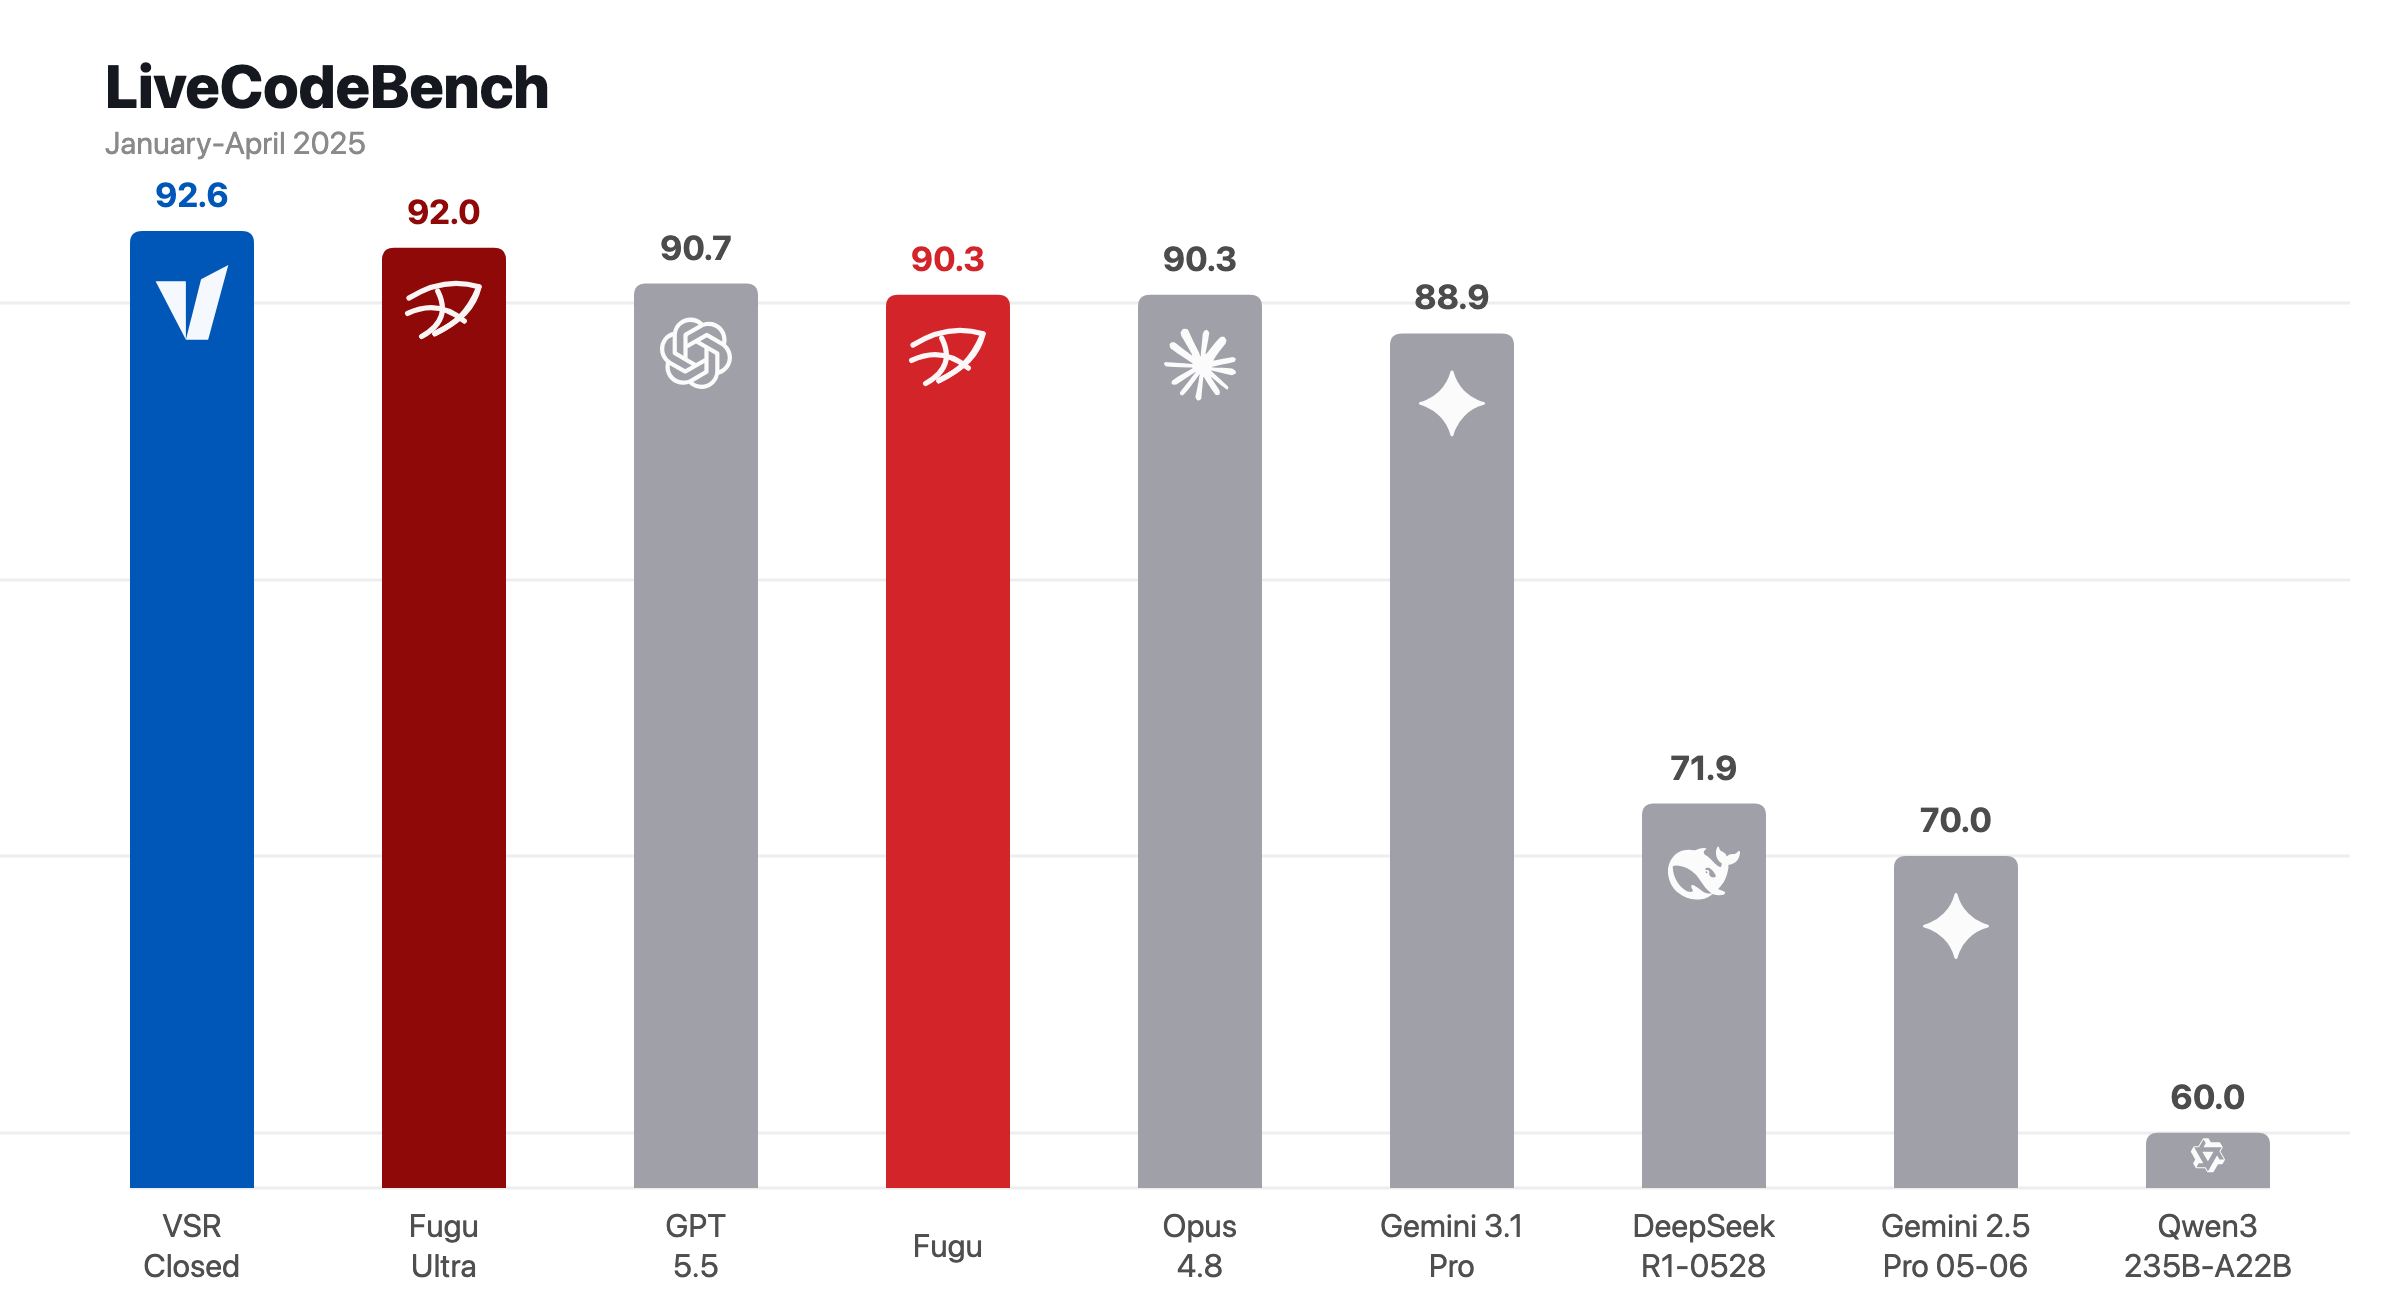
\includegraphics[width=0.27\paperwidth,trim=0 0 1080bp 0,clip]{figures/fig6_livecodebench_scorecard.png}%
    \hspace{0.03in}%
    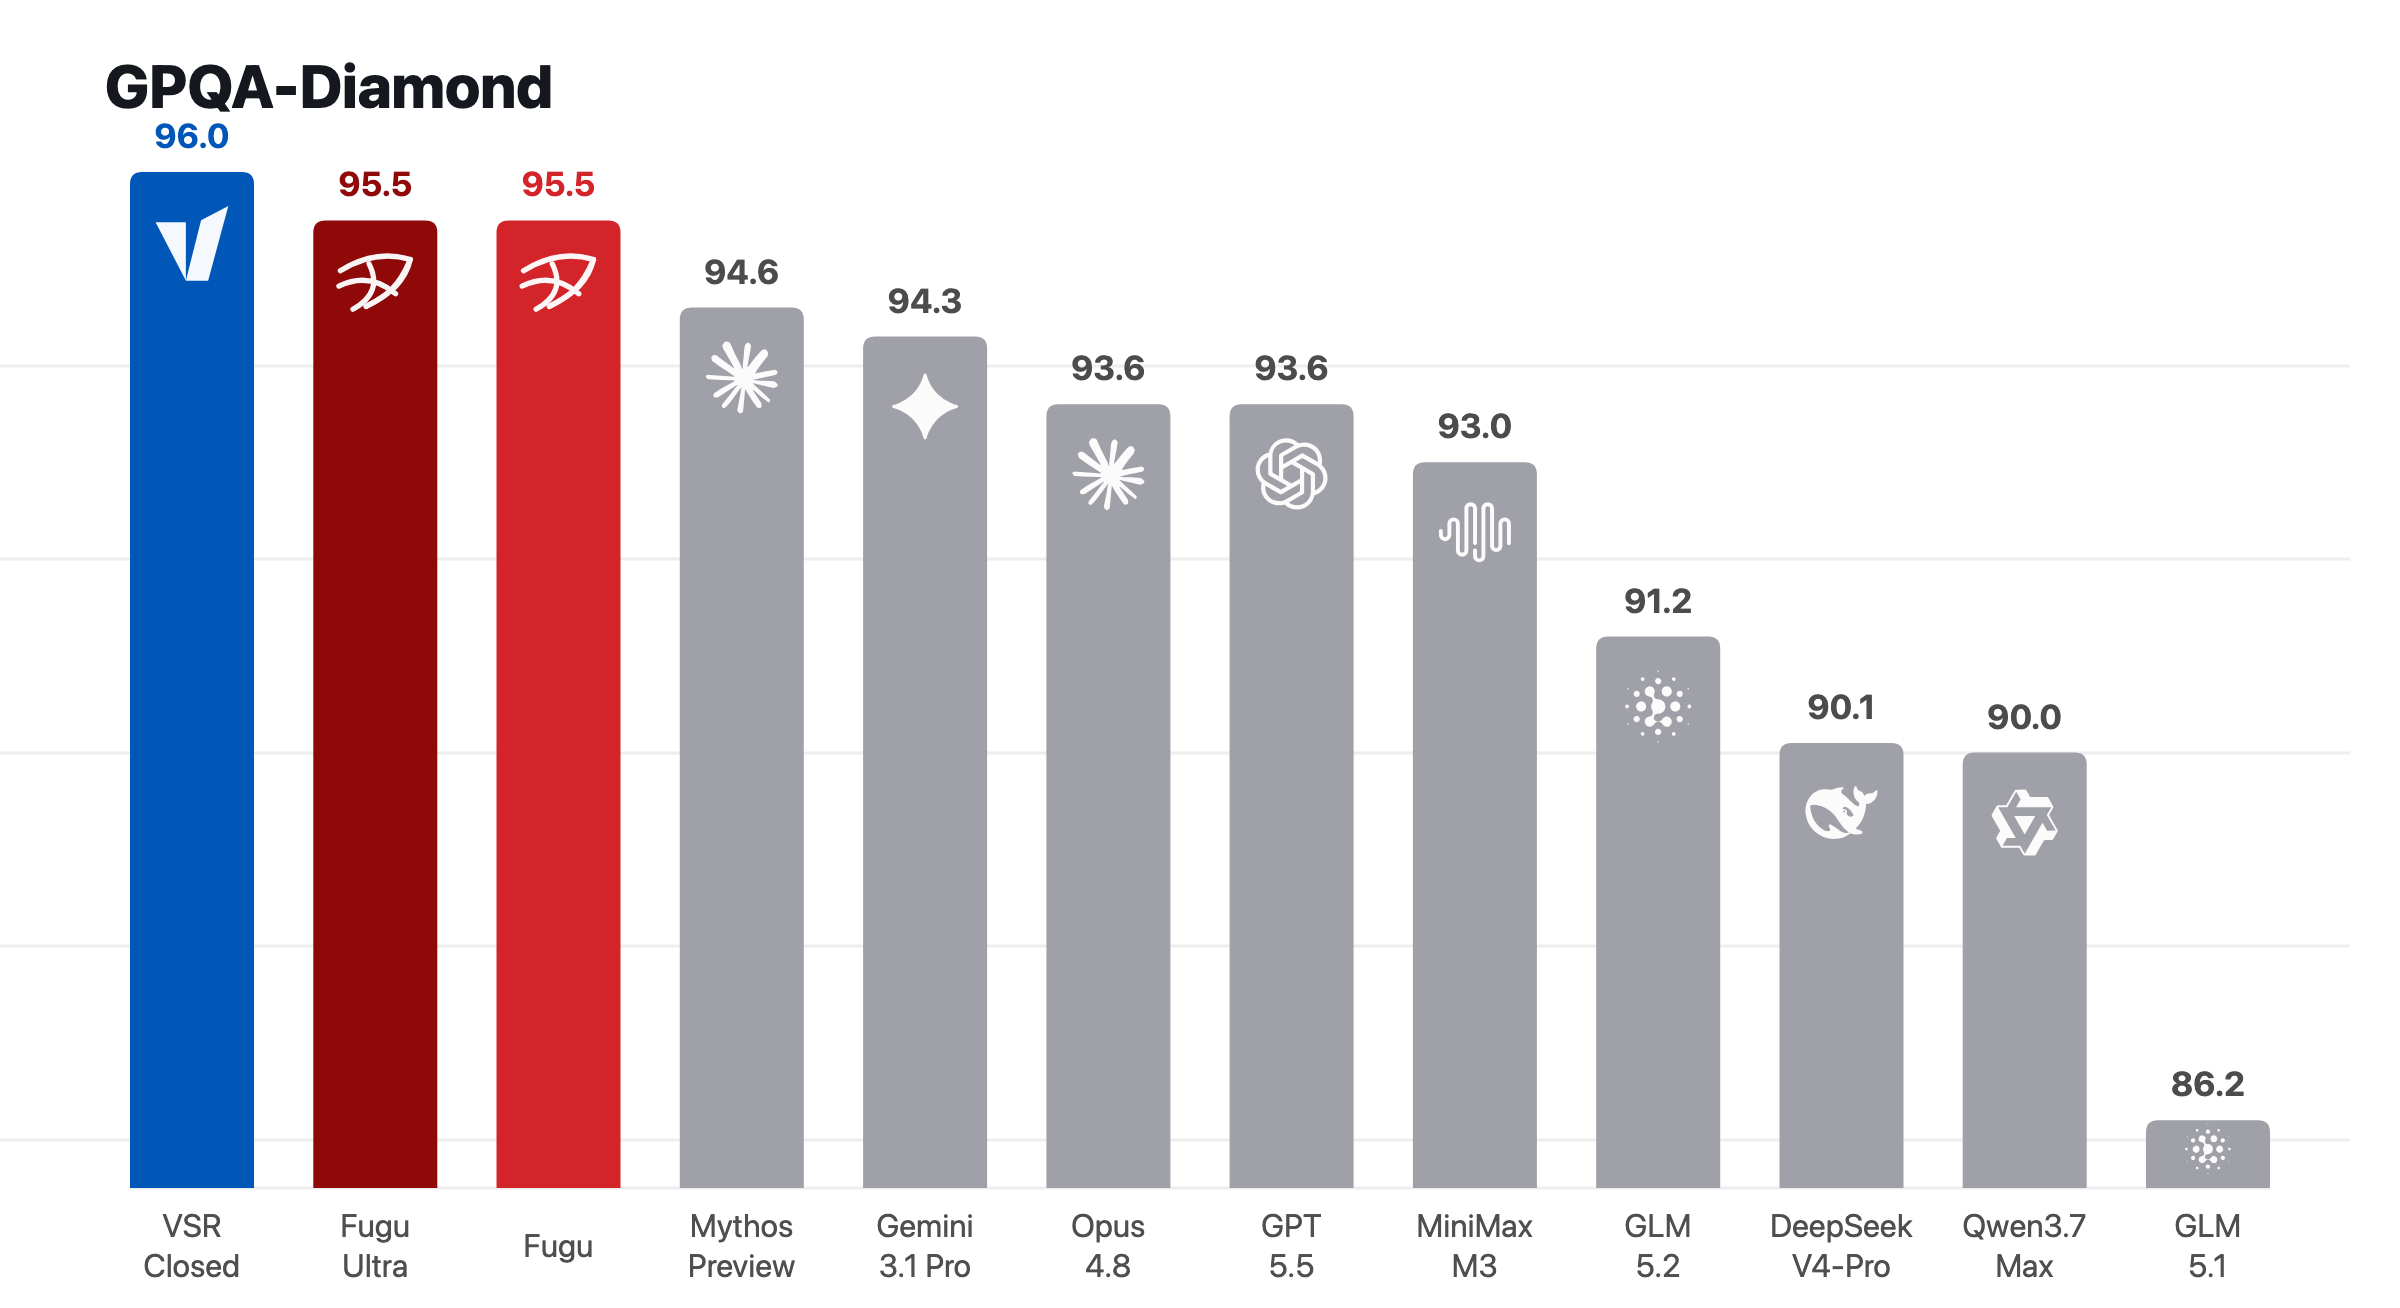
\includegraphics[width=0.27\paperwidth,trim=0 0 1035bp 0,clip]{figures/fig6_gpqa_scorecard.png}%
    \hspace{0.03in}%
    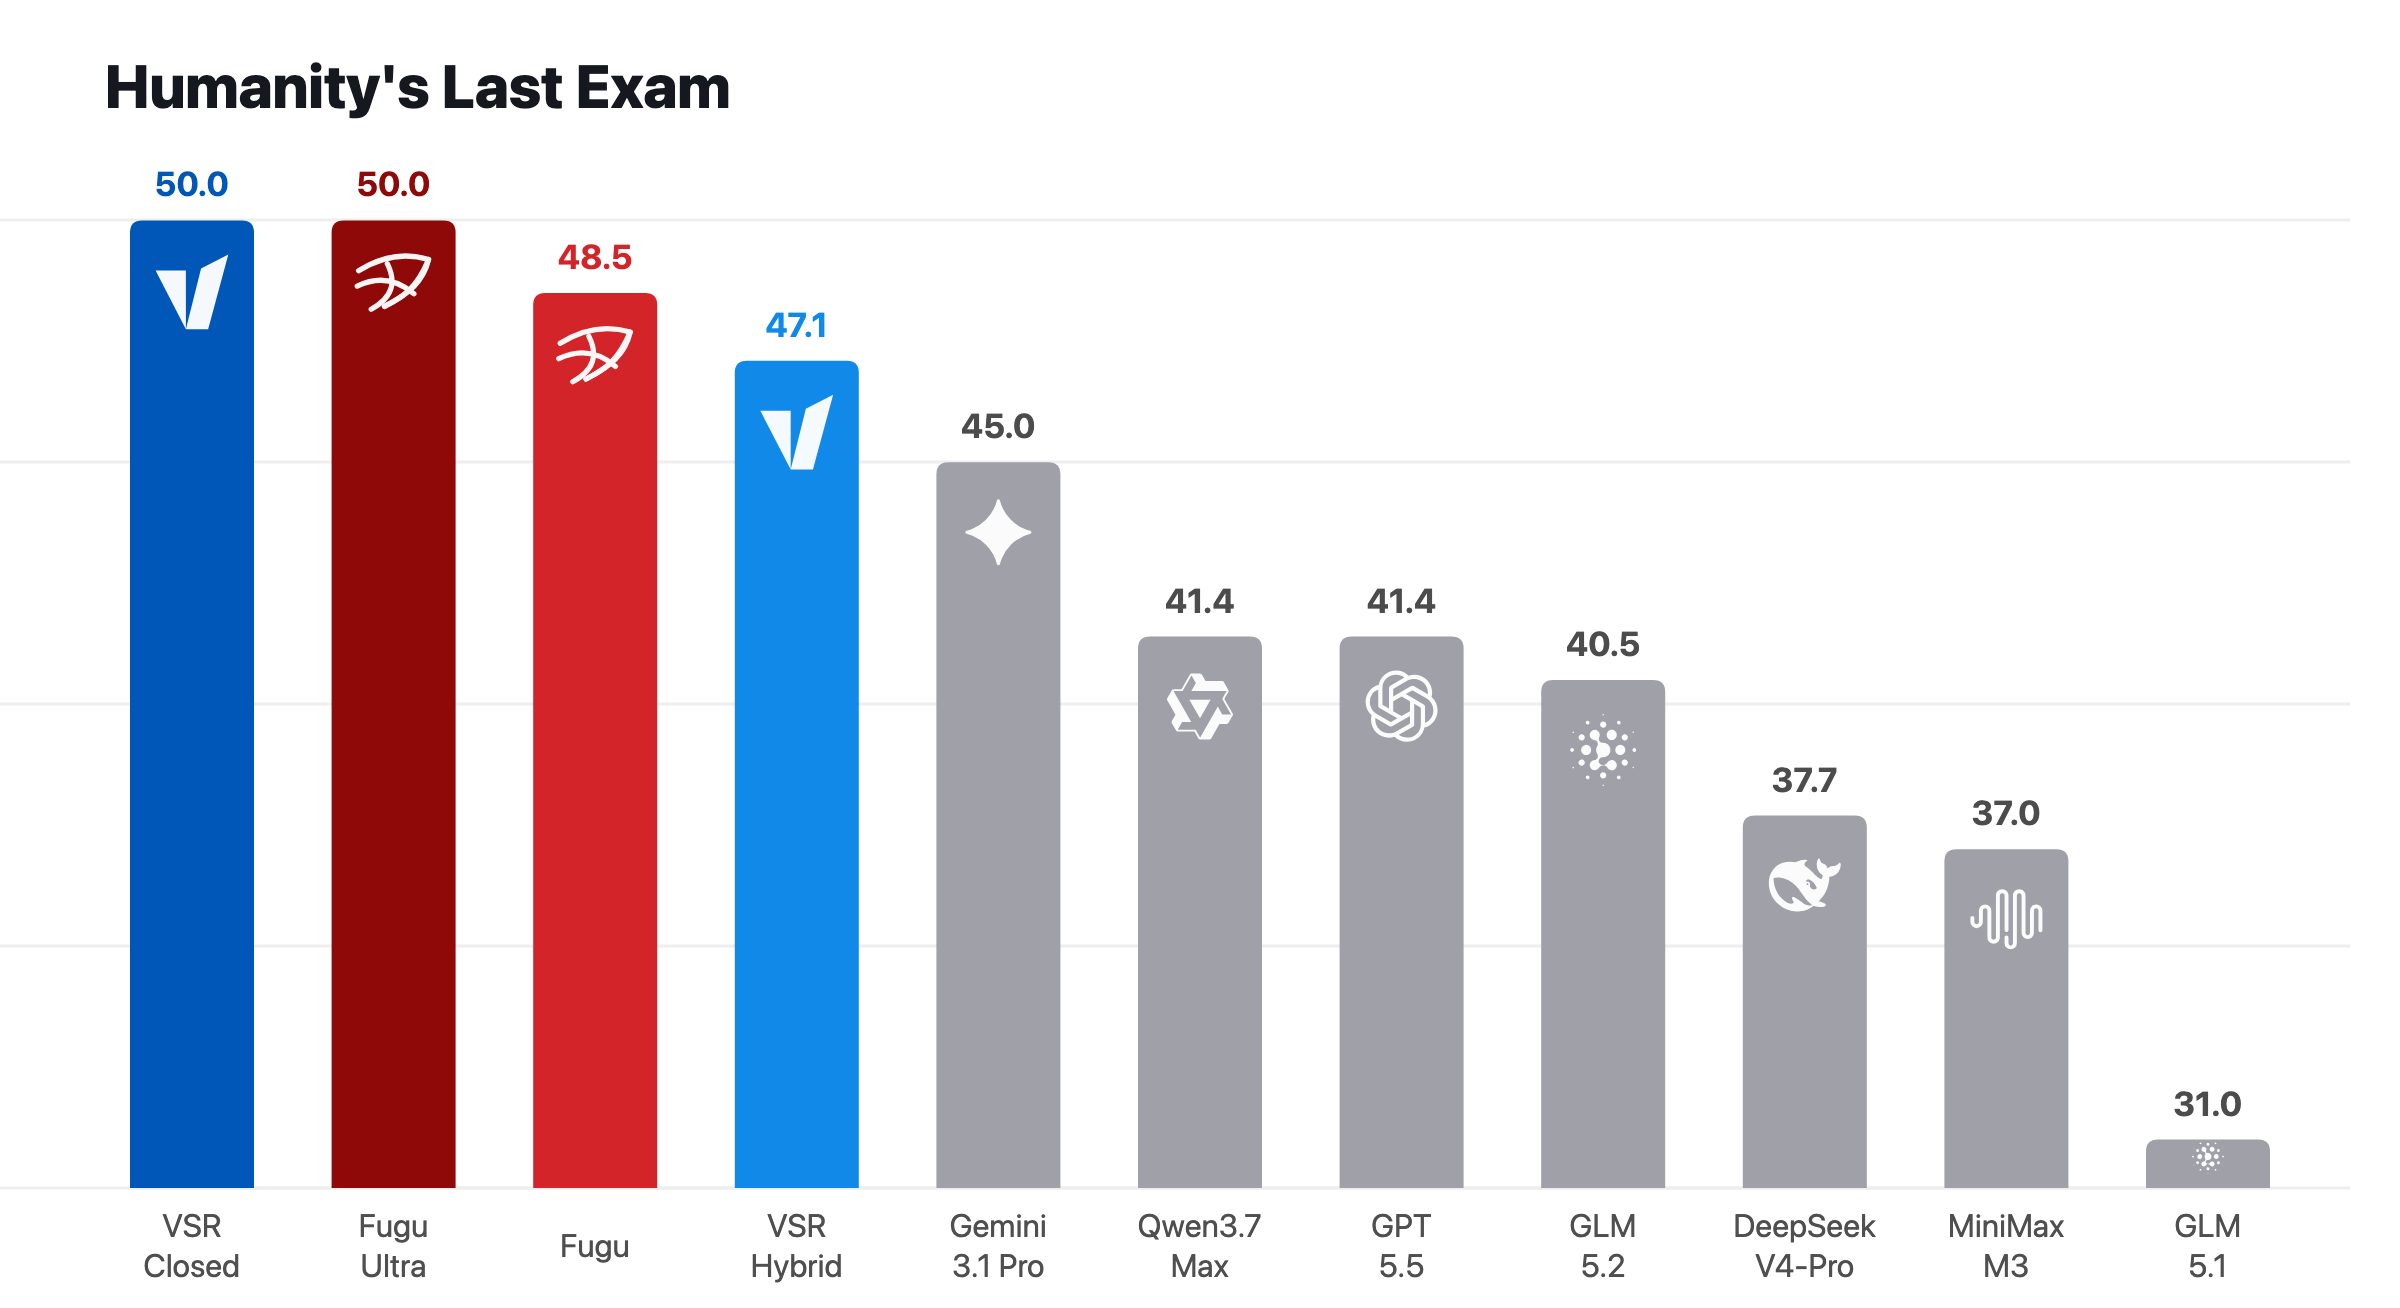
\includegraphics[width=0.27\paperwidth,trim=0 0 1080bp 0,clip]{figures/fig7_hle_scorecard.png}%
  }
  \caption{\textbf{Leading entries from the released accuracy-first MoM
  scorecards.} \emph{VSR Closed} denotes a realization using closed
  constituents; \emph{VSR Hybrid} combines open and closed constituents. GPQA
  uses the formal-50 slice, LiveCodeBench the 175-item January--April 2025
  slice, and HLE a 2,158-item text-only filter. These are protocol-specific
  release snapshots, not a matched-budget comparison
  \citep{vllm_sr_2026_microagent,tang_2026_fugu_v1}.}
  \label{fig:accuracy-scorecards}
\end{figure}

These runs exercise bounded deliberation and synthesis rather than the entire
action algebra. Looper metadata records models used and call counts. Router
Replay and usage records provide aggregate decision, token, and cost data,
while runtime metrics provide latency observability. The canonical per-call
event trace required for strict matched-budget comparison is part of the
proposed evaluation contract.

Figure~\ref{fig:accuracy-scorecards} reproduces the broader scorecard context in
which the results were released. It also includes prior project-reported HLE
closed and hybrid aggregates over a 2,158-item text-only filter
\citep{phan_2026_hle}. Those HLE rows are retained as a released system snapshot;
the current versioned evaluation manifest covers GPQA and LiveCodeBench. Public
reference bars use source-specific protocols and provide context, not a
matched-budget baseline. In particular, the LiveCodeBench and text-only HLE
comparators are pinned to the 175-item and 2,158-item protocols reported with
Fugu v1 rather than the later full-benchmark revision
\citep{tang_2026_fugu_v1}. The figure therefore illustrates that MoM admits an
accuracy-first operating point; it is not the controlled scaling comparison.

\FloatBarrier
\subsection{Routing-aware fleet planning}

Logical routing changes the workload presented to the serving fleet. To
illustrate the connection, an analytical two-pool planner replays the
request-length distribution from LMSYS-Chat-1M, a real-world conversation
dataset collected partly through Chatbot Arena
\citep{zheng_2023_lmsyschat,chiang_2024_chatbotarena}, at 100 requests per
second. The homogeneous estimate assigns all traffic to a 65K-context 70B
profile and yields 14 A100 GPU-equivalents of continuous capacity. A
length-aware split between 4K- and 65K-context pools estimates 8 A100
GPU-equivalents under the same 500 ms time-to-first-token target. At the
planner's assumed \$2.21 per GPU-hour, annualized cost changes from
approximately \$271K to \$155K, a 42.9\% simulated reduction.

This case study instantiates Workload--Router--Pool coupling: the trace policy
shapes the demand seen by each pool, so capacity planning cannot be an
afterthought to model selection \citep{chen_2026_wrp}. Once routing probabilities
and context requirements are explicit, placement and capacity become
optimization variables rather than hidden endpoint properties. The numbers are
analytical capacity estimates, not a production-cluster measurement;
deployment studies must calibrate the planner and repeat the comparison across
hardware, providers, and failure conditions.

\FloatBarrier
\subsection{The controlled scaling test}
\label{sec:required-experiments}

The controlled scaling experiment fixes a benchmark and constructs nested pools
of increasing size and capability diversity. At each size, it compares the
strongest constituent, learned selection, a fixed panel, an adaptive MoM, and an
oracle selector under matched call, token, cost, or latency budgets. It reports
oracle headroom, controller realization, per-item error correlation, topology
activation, contract failures, and repeated-run uncertainty. This design
separates conditional capacity from the effect of spending more inference
compute. Section~\ref{sec:limitations} extends the test to portability,
adaptation, sovereignty, and governance. Figure~\ref{fig:matched-budget-protocol}
summarizes the comparison.

\begin{figure}[H]
  \centering
  \resizebox{\linewidth}{!}{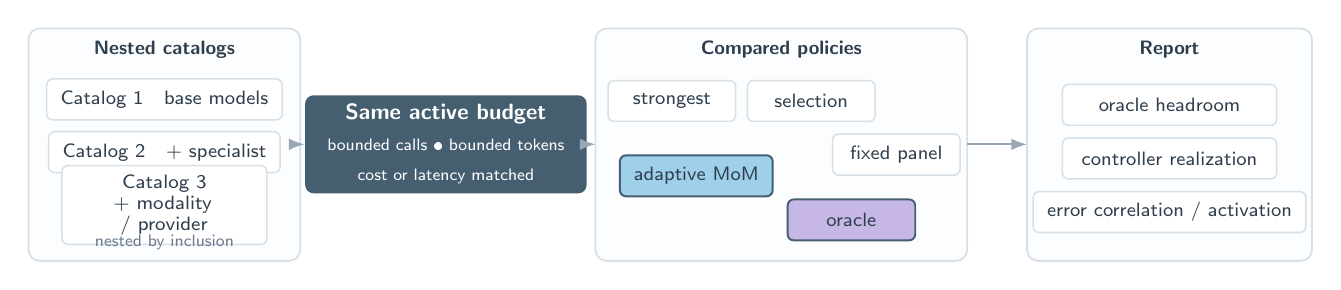
\begin{tikzpicture}[
  x=1cm,y=1cm,font=\sffamily,>=Latex,
  flow/.style={-{Latex[length=2.0mm]},draw=MoMGray,line width=0.70pt},
  group/.style={draw=MoMBorder,fill=MoMBlueLight!10,rounded corners=4pt,
    line width=0.65pt},
  card/.style={draw=MoMBorder,fill=white,rounded corners=2.2pt,
    line width=0.55pt,minimum height=0.52cm,inner xsep=5pt,align=center,
    font=\sffamily\fontsize{6.8}{7.6}\selectfont,text=MoMText},
  core/.style={draw=none,fill=MoMDark,text=white,rounded corners=3pt,
    minimum height=1.15cm,inner xsep=8pt,align=center},
  active/.style={card,draw=MoMDark,fill=MoMBlue,line width=0.72pt},
  oracle/.style={card,draw=MoMDark,fill=MoMPurple,line width=0.68pt},
  title/.style={font=\sffamily\bfseries\fontsize{7.5}{8.3}\selectfont,
    text=MoMText},
  muted/.style={font=\sffamily\fontsize{6.2}{7.0}\selectfont,text=MoMMuted}
]

% One left-to-right evaluation protocol. No curve is shown because this is a
% measurement design, not an empirical result.
\draw[group] (0.00,0.20) rectangle (3.45,3.15);
\node[title] at (1.725,2.88) {Nested catalogs};
\node[card,minimum width=2.55cm] at (1.725,2.25)
  {Catalog 1\quad base models};
\node[card,minimum width=2.55cm] at (1.725,1.58)
  {Catalog 2\quad + specialist};
\node[card,text width=2.25cm,minimum height=0.64cm] at (1.725,0.91)
  {Catalog 3\\+ modality / provider};
\node[muted] at (1.725,0.43)
  {nested by inclusion};

\node[core,minimum width=2.70cm] (budget) at (5.30,1.68)
  {{\bfseries\fontsize{8.0}{8.8}\selectfont Same active budget}\\[-1pt]
   {\fontsize{6.5}{7.2}\selectfont bounded calls \textbullet\ bounded tokens}\\[-1pt]
   {\fontsize{6.2}{6.9}\selectfont cost or latency matched}};

\draw[group] (7.20,0.20) rectangle (11.92,3.15);
\node[title] at (9.56,2.88) {Compared policies};
\node[card,minimum width=1.62cm] at (8.17,2.23) {strongest};
\node[card,minimum width=1.62cm] at (9.94,2.23) {selection};
\node[card,minimum width=1.62cm] at (11.02,1.55) {fixed panel};
\node[active,minimum width=1.90cm] at (8.48,1.28) {adaptive MoM};
\node[oracle,minimum width=1.62cm] at (10.45,0.72) {oracle};

\draw[group] (12.68,0.20) rectangle (16.30,3.15);
\node[title] at (14.49,2.88) {Report};
\node[card,minimum width=2.72cm] at (14.49,2.18) {oracle headroom};
\node[card,minimum width=2.72cm] at (14.49,1.50) {controller realization};
\node[card,minimum width=2.72cm] at (14.49,0.82)
  {error correlation / activation};

\draw[flow] (3.45,1.68) -- (budget.west);
\draw[flow] (budget.east) -- (7.20,1.68);
\draw[flow] (11.92,1.68) -- (12.68,1.68);

\end{tikzpicture}
}
  \caption{\textbf{Matched-budget protocol for MoM scaling.} Nested catalogs
  are evaluated under one active-work envelope. Comparing a strongest
  constituent, learned selection, a fixed panel, an adaptive MoM, and an oracle
  separates catalog complementarity from controller realization and additional
  inference work. The diagram specifies an evaluation protocol, not a result.}
  \label{fig:matched-budget-protocol}
\end{figure}

\FloatBarrier

\section{Related Architectures}
\label{sec:related}

\paragraph{Conditional computation inside a model.}
Adaptive mixtures and conditional-computation methods established the use of a
learned gate to allocate examples to specialized computation
\citep{jacobs_1991_mixture,bengio_2013_conditional}. Sparsely gated
Mixture-of-Experts (MoE), GShard, and Switch Transformers scale that principle
while activating only a subset of parameters for each input
\citep{shazeer_2017_moe,lepikhin_2020_gshard,fedus_2021_switch}. Their experts
typically share a checkpoint, training loop, tensor interface, and deployment
boundary. MoM retains conditional computation but moves the boundary outward:
a constituent can be an independently versioned local model, a private
specialist, or a closed remote service. MoM does not require joint
differentiability and often forgoes it; in return, it permits independent
evolution, heterogeneous placement, and explicit policy and failure boundaries.

\paragraph{Cascades and model routing.}
Cost-aware cascades and learned routers choose among models under quality and
resource objectives
\citep{aggarwal_2023_automix,chen_2023_frugalgpt,ding_2024_hybrid,
ong_2024_routellm}; RouterBench supplies a routing evaluation framework
\citep{hu_2024_routerbench}. Model-GLUE instead studies model selection and
parameter or output aggregation over a model zoo \citep{zhao_2024_modelglue}.
These methods provide important controllers and protocols. A general MoM also
admits parallel calls, verification, synthesis, and bounded workflows, and
places contracts and deployment identity inside the model lifecycle.

Closer whole-model precedents route among domain specialists, train asynchronous
language-model mixtures, form domain-specific consensus, or orchestrate models
and agents \citep{simonds_2024_modem,filippova_2025_smalltalk,
wang_2025_telemom,guo_2025_moma,pecerskis_2026_nsed}. Brick and NSED
independently use the Mixture-of-Models name; HyDRA and RouteBalance study
closely related capability routing and serving-aware scheduling
\citep{massa_2026_brick,garg_2026_hydra,da_2026_routebalance}. Fugu is a
particularly close contemporary system: trained orchestrator models dynamically devise
agentic scaffolds over a model team and expose the result through a model-like
interface \citep{tang_2026_fugu}. Our focus is the open infrastructure boundary
around such behavior---a finite execution algebra, portable identity,
environment binding and lock, attributable traces, and one lifecycle across
training, evaluation, and serving.

\paragraph{Ensembles and inference-time collaboration.}
Ensembling, response fusion, and Mixture-of-Agents exploit complementary outputs
from several models \citep{jiang_2023_llmblender,wang_2024_moa,li_2025_selfmoa}.
The cited methods evaluate a fixed composition topology. In our formulation,
parallel deliberation is one topology in a larger trace space, and a controller
may choose another under explicit resource and policy constraints. The trace
also makes its additional inference compute visible.

\paragraph{Compound AI systems and language-model programming.}
Compound AI systems frame application intelligence as the interaction of
models, retrieval, tools, and control logic \citep{kandogan_2024_compound}.
Language-model programming systems likewise provide constraints, control flow,
optimization, and efficient execution for multi-call programs
\citep{beurerkellner_2022_lmql,khattab_2023_dspy,zheng_2023_sglang}.
MoM narrows that broad systems view into a model-facing abstraction with a
bounded graph, explicit optimization variables, and portable identity. An agent
can invoke a MoM or request a bounded workflow, while the infrastructure layer
retains authority over admissibility and accounting. Programming systems can be
authoring frontends or execution backends; they do not by themselves define the
deployment identity proposed here.

\paragraph{Serving graphs, model packages, and runtimes.}
KServe InferenceGraph offers declarative sequence, switch, ensemble, and splitter
nodes behind one endpoint \citep{kserve_2026_inferencegraph}. Hugging Face model
repositories offer revisioned model coordinates; MLflow packages signatures and
loading flavors; and OCI manifests provide content-addressed distribution
\citep{huggingface_2026_models,mlflow_2026_model_format,
oci_2025_image_spec}. ONNX most clearly separates a typed model IR from
capability-negotiated execution providers
\citep{onnx_2026_ir,onnxruntime_2026_execution_providers}, while GGUF exemplifies
a self-describing materialized edge artifact \citep{gguf_2026_spec}. None alone
defines a composite model whose constituents may also be closed services. The
proposed lifecycle retains native leaf formats while adding a
preference-conditioned trace distribution, hard admissibility, separate
logical and physical identities, and trace-linked evidence. Serving runtimes
address complementary memory management, model multiplexing, scheduling and
migration, and multi-tenant adapter serving; examples include vLLM, MuxServe,
Llumnix, and Punica
\citep{kwon_2023_vllm,duan_2024_muxserve,sun_2024_llumnix,chen_2023_punica}.
A MoM artifact can bind to these systems without embedding mutable endpoints or
credentials.

\paragraph{Evolution of vLLM Semantic Router.}
Prior project papers developed signal-driven routing, workload--router--pool
optimization, a routing policy DSL, and agent orchestration
\citep{liu_2026_semanticrouter,chen_2026_wrp,liu_2026_conflictfree,chen_2026_orchestration}.
The earliest of these used ``MoM'' for mixture-of-modality deployments; here,
modality is one dimension of the broader catalog of independently versioned
models. Those mechanisms remain components of the reference engine. This paper
changes the unit of analysis from a routing decision to a versioned logical
model whose learned and authored state spans a pool, a control policy, an execution
topology, and contracts, together with an explicit deployment binding.

\section{Limitations and Research Agenda}
\label{sec:limitations}

The architecture covers finite, typed, resource-bounded graphs; it does not
make unbounded agency safe or guarantee a feasible binding. Mutable closed
services limit exact replay, the current system results do not establish the
matched-budget scaling hypothesis, and cross-provider or CPU--GPU--NPU portability
still requires controlled validation. Security, sovereignty, and grounding are
only as reliable as their evidence, enforcement, and checkers. Within those
boundaries, the research agenda rests on four claims with concrete validation
criteria.

\paragraph{Useful scale is complementarity at fixed active compute.}
A larger pool matters only when it adds capability, failure, resource, or
deployment diversity that a learned policy can exploit within the same call,
token, cost, energy, or latency budget. Matched-budget studies must therefore
report the strongest constituent,
oracle headroom, controller realization, repeated runs, error correlations, and
topology ablations as specified in Section~\ref{sec:required-experiments}.
Parallel panels and additional rounds count as active compute, not hidden model
capacity. The scaling curve of interest is attainable utility against catalog
diversity and active work; merely spending more inference is not conditional
scaling.

\paragraph{Logical model identity must survive physical change.}
If a MoM is to move between a robot, an edge site, a sovereign cluster, and a
managed service, its semantics cannot be identified with any one endpoint or
runtime. The bundle therefore implies a shared conformance suite:
canonicalization, signatures, operator capability negotiation, compatibility
tests, and independent engine implementations. A binder and resolver may
rebind logical references across CPU, GPU, NPU, and provider environments, but
every substitution must remain visible in the binding, lock, and evaluation. This is
especially important for mutable services whose weights, safety layers, prices,
limits, or aliases can change without exposing a checkpoint hash; a lock
records the best available evidence, while canaries and explicit revalidation
measure the remaining drift.

\paragraph{Lifecycle optimization must coordinate logical and physical state.}
Signals, control policies, pools, prompts, topologies, contracts, and placements
are optimized from different evidence and evolve on different timescales. Improving one in
isolation can destabilize another: a more aggressive gate changes fleet load,
a new binding changes latency and fallback behavior, and a new judge can change
the apparent reward. MoM lifecycle optimization therefore needs artifact- and
binding-level promotion, chronological evaluation, invariants, and rollback
\citep{chen_2026_wrp}. The research target is not convergence of one controller,
but stable improvement of realized utility and constraint satisfaction under
deployment drift.

\paragraph{Sovereignty and governance are properties of the trace.}
Sovereignty is not a binary choice between a local model and a public cloud.
Real deployments combine devices, jurisdiction-bound data centers, regional
providers, open weights, and selectively approved global services. Their
requirements span data and model control, residency, encryption-key control,
operations, supply chain, audit, and exit paths
\citep{european_commission_2026_sovereignty}. A MoM compiler should translate
such a profile into typed admissibility constraints over models, operators,
data paths, and bindings; cloud fallback must never silently override them.
The same principle applies to security, grounding, and preference governance.
Signals can guide execution but do not prove confidentiality or factuality,
and aggregate utility can hide systematically poor service for a group.
Least-privilege operators, secret separation, explicit boundary crossings,
per-group constraints, and worst-case evaluation make governance inspectable
on the realized trace rather than aspirational at the endpoint.

Progress on these four claims would turn model composition from a collection of
recipes into a model ecosystem with measurable scaling behavior, portable
identity, and a durable lifecycle.

\section{Conclusion}
\label{sec:conclusion}

Mixture-of-Models moves conditional computation from parameters within one
checkpoint to execution across independently versioned models. We define the
served object as a preference-conditioned distribution over finite, typed
traces, with hard admissibility, portable logical identity, and
environment-specific binding. Selection, cascades, fusion, multi-round
collaboration, and bounded workflows are model topologies rather than
application glue. The resulting intelligence is system-level: it arises from
co-designing the trace distribution with its physical realization, not from any
constituent or control component in isolation.

\vsr{} shows that an execution-facing subset of this abstraction can be
declarative and executable without joint access to constituent weights. The
portable bundle, lock, and conformance suite define its next implementation
boundary. The central empirical question is whether added model diversity
increases utility under matched active compute. If it does, model runtimes will
need to execute and evolve composite models across providers, jurisdictions,
devices, and fleets as reliably as they execute checkpoints across machines.
The resulting mission is to make virtual composite models buildable,
evaluable, portable, and servable with the same rigor as checkpoints.


\bibliography{references}
\bibliographystyle{iclr2026_conference}

\appendix
\section{Experimental Protocol}
\label{app:reproducibility}
\begingroup
\small

This appendix records the protocol behind Section~\ref{sec:evidence} and the
evidence needed to audit an end-to-end system result. The current versioned
evaluation manifest covers GPQA-Diamond and LiveCodeBench; the HLE description
corresponds to the prior released scorecard retained in
Figure~\ref{fig:accuracy-scorecards}. The open reference implementation is available at
\url{https://github.com/vllm-project/semantic-router}. The evaluated
configurations were served through an OpenAI-compatible endpoint under the
shared alias \texttt{vllm-sr/auto}; each benchmark configuration nevertheless
has a distinct pool and topology and should be released under its own immutable
coordinate and digests.

\subsection{Constituent pools and trace budgets}

\paragraph{GPQA-Diamond.}
The benchmark is GPQA-Diamond~\citep{rein_2023_gpqa}.  The evaluated MoM
uses Gemini 3.1 Pro Preview, GPT-5.5, and Claude Opus 4.8.  Each request launches
one reasoning call to each constituent and then invokes Gemini for synthesis,
for four nominal model calls.  The output contract admits exactly one answer in
\{A,B,C,D\}.  The reported run contains 50 questions and is labeled
\emph{formal-50} to distinguish it from the complete 198-question benchmark.

\paragraph{LiveCodeBench.}
The evaluated window uses LiveCodeBench~\citep{jain_2024_livecodebench} v6,
January--April 2025, with 175 problems.  The pool again contains Gemini 3.1 Pro
Preview, GPT-5.5, and Claude Opus 4.8. Request signals select one of two
principal traces. The first uses three analysis calls followed by GPT-5.5
synthesis, for four calls in total; the second uses five breadth calls followed
by GPT-5.5 synthesis, for six calls in total. The contract requires one complete
Python solution with the problem's function or standard-input interface
preserved.  Sandboxed execution provides the task score.  Five missing
generations are assigned zero credit, so the denominator remains 175.

\paragraph{Humanity's Last Exam.}
The released scorecard reports a text-only filter over the 2,500-item release
of Humanity's Last Exam (HLE)~\citep{phan_2026_hle}, with 2,158 retained items.
The closed realization contains Claude Opus 4.8 and Gemini 3.1
Pro Preview. Depending on request risk, it obtains two, three, or four candidate
responses and then invokes Gemini for synthesis, for three to five nominal
calls; its scoring judge is also Gemini 3.1 Pro Preview. The hybrid realization
contains two independent GLM-5.2 sampling roles, GPT-5.5, Claude Opus 4.8, and
Gemini 3.1 Pro Preview. It obtains three or four candidate responses and then
invokes Gemini for synthesis, for four or five nominal calls.
The contract requires an explanation, exact answer, and calibrated confidence
field. The hybrid scoring path uses GPT-5.5. In both realizations, the judge
identity may also participate in the execution graph, so the reported numbers
are end-to-end system scores; comparisons intended to isolate constituent
quality should instead use a disjoint judge pool and report multi-judge
agreement.

For archival reproduction, each dataset must be pinned by repository revision,
configuration, filter predicate, ordered item identifiers, and an identifier
digest. In particular, \emph{LiveCodeBench v6} here denotes the 175-item
January--April 2025 configuration rather than the cumulative
\texttt{release\_v6}; the HLE count is produced by the text-only filter rather
than a benchmark-defined split; and the GPQA formal-50 item list requires an
explicit selection record. These public benchmarks predate the evaluated 2026
constituents, so no result is interpreted as contamination-free
generalization.

All constituent calls in these three experiments use the same managed model
gateway.  Thus the experiments test heterogeneous model identities and trace
topologies, while cross-provider and cross-hardware portability remain separate
evaluation dimensions.

\subsection{Request, trace, and scoring records}

A reproducible and independently auditable MoM evaluation requires more than
final predictions. Each
request record should contain:

\begin{itemize}
  \item dataset version, split, immutable example identifier, and input digest;
  \item logical MoM identity, behavior variant, request preference, bundle digest, and deployment-lock
  digest;
  \item signals, projection values, matched decision, selected topology, and
  hard-constraint outcomes;
  \item every constituent model and service revision, prompt digest, sampling
  parameters, retry index, stop reason, and terminal status;
  \item raw response or policy-compliant encrypted/redacted equivalent, parsed
  answer, contract-validation result, repair, fallback, and abstention events;
  \item input, cached-input, reasoning, and output token counts when available;
  \item per-call and end-to-end latency, timeouts, rate limits, and failures;
  \item realized monetary and, where estimable, energy cost under the declared
  accounting model;
  and
  \item scorer and judge versions, raw score, aggregation rule, and uncertainty.
\end{itemize}

Run-level metadata should additionally record engine and dependency versions,
model inventory, start and end times, concurrency, seeds, counts of attempted,
completed, and missing items, and checksums for every output shard. A run is complete
only when the expected item identifiers and denominator match; the presence of
an aggregate score file alone is insufficient.

\subsection{Routing-aware fleet-planning protocol}

The capacity example uses the empirical request-length distribution from
LMSYS-Chat-1M, collected partly through Chatbot
Arena~\citep{zheng_2023_lmsyschat,chiang_2024_chatbotarena}, at an arrival rate
of 100 requests per second and a 500 ms time-to-first-token target. The modeled
worker serves a 70B model with eight-way tensor parallelism on A100 GPUs. The
homogeneous baseline assigns every request to a 65K-context pool.  The routed
plan assigns short requests to a 4K-context pool and long requests to the 65K
pool, then sweeps the threshold subject to the same latency target.  GPU cost is
fixed at \$2.21 per hour.  Both reported plans are continuous analytical
capacity estimates before rounding to whole eight-GPU workers; they are not
deployable cluster counts or measurements from a production cluster.

For deployment use, the planner should first be calibrated against observed
prefill/decode throughput and tail latency, then validated on held-out traces.
A complete study should repeat the sweep over arrival processes, context
distributions, SLOs, accelerator types, model profiles, failures, and price
assumptions, and should compare analytical predictions with discrete-event and
live-cluster measurements.

\subsection{Release contract}

An independently checkable release should publish the canonical MoM bundle,
deployment binding and lock, constituent inventory, prompts, contracts,
benchmark manifests, per-item traces, and deterministic report generator.
Credentials, authorization headers, and private request content must never be
embedded; secret references and policy-preserving redaction retain the logical
identity needed for verification.  All tables and figures should be regenerated
from immutable request and run records, and their reported digests should match
the released artifacts.
\endgroup

\section{Proposed MoM Bundle Format}
\label{app:artifact-profile}
\begingroup
\footnotesize

This appendix instantiates the artifact contract in
Section~\ref{sec:artifact}. The format is a versioned proposal; a
machine-readable companion supplies schemas for the manifest, typed IR,
realization profile, binding, lock, evaluation protocol, evaluation
attestation, and run record, together with one verified example.

\subsection{Bundle contents and evidence boundary}

The manifest is an immutable index over the human model coordinate, behavior
variant, semantic digest, typed entrypoints, canonical specification, semantic
assets, contracts, evaluation protocols, and optional realization templates.
Canonical IR remains the sole semantic authority. Authoring source and model
cards are optional distribution objects rather than executable authorities.
Evaluation results, signatures, SBOMs, and build provenance are separate
digest-bound attestations: publishing new evidence does not change the model
being evaluated.

Every object descriptor contains a normalized relative path, media type,
SHA-256 digest, and byte size. Absolute, backslash, empty, dot, repeated,
traversal, and symlink paths are rejected before parsing. A production archive
importer must additionally bound expanded size, file count, nesting, and
compression ratio and reject hard links, devices, and other non-regular files.

The example exposes one accuracy-first model and two realization profiles:
ROCm plus cloud and CUDA plus cloud. Behavior variants belong to logical
identity; realization profiles contain endpoint-free compatibility
requirements and do not. A binding chooses one realization profile and supplies
concrete candidates.

\subsection{Four identities without circular hashes}

Let $C$ be canonical JSON and $H$ be SHA-256. Let $I$ be the fully defaulted and
typed IR, whose semantic assets are themselves content-addressed. Let $M$ be
the manifest, whose object descriptors commit to the distributed byte closure.
Let $N(B_s)$ be the normalized typed representation obtained from binding
source $B_s$, and let $L$ be the completed normalized lock. The four identities
are
\begin{equation}
 \begin{aligned}
 d_{\mathrm{semantic}} &= H(C(I)),&
 d_{\mathrm{bundle}}   &= H(C(M)),\\
 d_{\mathrm{binding}}  &= H(C(N(B_s))),&
 d_{\mathrm{lock}}     &= H(C(L)).
 \end{aligned}
 \label{eq:bundle-identities}
\end{equation}
No object stores its own digest. The manifest stores
$d_{\mathrm{semantic}}$; the binding stores semantic and bundle subjects; the
lock stores that subject and $d_{\mathrm{binding}}$; traces and attestations
then store all four. Formatting a YAML binding therefore cannot create a new
environment identity.

\subsection{Target compatibility and locking}

A logical constituent declares an identity and required or preferred
capabilities, including protocol, modality, interface features, input and
output limits, and data policy. A realization profile may additionally require
a wire transport, API adapter, serving runtime, leaf-artifact format,
accelerator API, vendor, architecture, or deployment driver. Environment policy may strengthen but
never relax semantic constraints. Resolution is thus the intersection of
logical admissibility, realization-profile requirements, and environment
policy.

The lock records the complete candidate inventory available to an execution,
not the one candidate selected by a particular request. For open artifacts it
may pin a content digest or repository revision together with tokenizer,
runtime image, protocol adapter, and accelerator evidence. For a closed service
it marks identity as observed-opaque, records an observation time and probe
digest, and makes no bitwise-reproducibility claim. Floating dependencies are
excluded from a production lock.

\subsection{Distribution closures and evaluation}

A thin export retains immutable external references; a materialized export
vendors leaf artifacts whose licenses permit redistribution; and a targeted
export additionally carries runtime objects for selected realization
profiles. Materialization fails for a closed provider rather than treating an
API alias as an offline model. A canonical directory and deterministic archive
define local exchange; OCI descriptors, manifests, and referrers provide a
natural registry transport and evidence attachment.

An evaluation protocol is part of the bundle because it defines an assessment
procedure. A result is an external attestation over semantic, bundle, binding,
lock, protocol, dataset, and harness digests, plus sampling and concurrency
settings. Serving and evaluation therefore consume the same resolved model
identity, while later measurements remain independently publishable.

\subsection{Conformance}

The companion verifier checks all supplied schemas; stable canonical
identities; traversal-safe paths, byte sizes, and digests; manifest/IR semantic
closure; behavior variants and realization profiles; graph reachability,
explicit contract branches, universal termination, and finite bounds; fail-closed hard
constraints; constituent identity and capability satisfaction; complete lock
inventory; pinned and observed-opaque evidence; secret non-inclusion; and run
and evaluation attribution to all four identities.

A complete cross-engine suite must additionally test deterministic compilation,
source-to-IR semantic preservation, operator capability negotiation, archive
hardening, license and extension trust, trace conformance, and portability
across at least two disclosed bindings while fixing semantic and bundle
digests.
\endgroup


\end{document}
